% !TEX program = xelatex
% Tarea #3 — Análisis formal del problema computacional complejo
% Compilación: XeLaTeX dos veces (xelatex main.tex), o latexmk -xelatex main.tex.
% No compila con pdfLaTeX porque usa fontspec.
\documentclass[11pt,a4paper,spanish]{article}

% Se compila con XeLaTeX para que los acentos del código de los anexos se
% lean directamente como UTF-8, sin conversiones.
\usepackage{fontspec}
\setmainfont{Latin Modern Roman}
\setsansfont{Latin Modern Sans}
\setmonofont{Latin Modern Mono}[Scale=MatchLowercase]
\usepackage[spanish,es-tabla,es-noquoting]{babel}
\usepackage[margin=2.5cm]{geometry}
\usepackage{graphicx}
\usepackage{booktabs}
\usepackage{array}
\usepackage{longtable}
\usepackage{tabularx}
\usepackage{multirow}
\usepackage{enumitem}
\usepackage{float}
\usepackage{caption}
\usepackage{xcolor}
\usepackage{titlesec}
\usepackage{fancyhdr}
\usepackage{setspace}
\usepackage{listings}
\usepackage[numbers]{natbib}
\usepackage{hyperref}

% --- Estilo de la página ---------------------------------------------------
\onehalfspacing
\setlength{\parindent}{1.2em}
\setlength{\parskip}{0.4em}
\setlength{\emergencystretch}{2em}

\titleformat{\section}{\large\bfseries}{\thesection}{0.8em}{}
\titleformat{\subsection}{\normalsize\bfseries}{\thesubsection}{0.8em}{}
\titleformat{\subsubsection}{\normalsize\bfseries}{\thesubsubsection}{0.8em}{}
\setcounter{secnumdepth}{3}
\setcounter{tocdepth}{3}
% La portada no lleva número; la numeración visible empieza en 2, como en la
% Tarea 2 y como los puntos que enumera el enunciado de la Tarea 3.
\setcounter{section}{1}

\setlength{\headheight}{14pt}
\pagestyle{fancy}
\fancyhf{}
\fancyhead[L]{{\small CCPG1044 --- Inteligencia Artificial}}
\fancyhead[R]{{\small Grupo 4 --- Tarea 3}}
\fancyfoot[C]{\thepage}
\renewcommand{\headrulewidth}{0.4pt}
\fancypagestyle{plain}{\fancyhf{}\fancyfoot[C]{\thepage}}

\hypersetup{colorlinks=true,linkcolor=black,citecolor=black,urlcolor=blue!70!black,
            pdftitle={Tarea 3 -- Analisis formal del problema}}
% La bibliografía lleva el número de sección 11 y aparece en el índice.
\renewcommand{\bibsection}{\section{\refname}}

% --- Código de los anexos --------------------------------------------------
\lstdefinestyle{codigo}{
  basicstyle=\ttfamily\footnotesize,
  breaklines=true,
  frame=single,
  rulecolor=\color{black!25},
  xleftmargin=1em,
  xrightmargin=1em,
  numbers=left,
  numberstyle=\tiny\color{black!60},
  stepnumber=1,
  showstringspaces=false,
  tabsize=4,
  extendedchars=true,
  captionpos=b,
  abovecaptionskip=6pt,
  belowcaptionskip=4pt
}
\lstdefinestyle{python}{style=codigo,language=Python}
\lstdefinestyle{plantuml}{style=codigo}
\lstset{style=codigo}

% ==========================================================================
\begin{document}

% ------------------------------------------------------------------ portada
\begin{titlepage}
\centering
{\large ESCUELA SUPERIOR POLITÉCNICA DEL LITORAL\par}
\vspace{0.4em}
{\large Facultad de Ingeniería en Electricidad y Computación --- FIEC\par}
\vspace{1.2em}
{\large Curso CCPG1044 --- Inteligencia Artificial\par}
\vspace{0.6em}
{\normalsize Paralelo 2\par}

\vspace{2.6cm}
{\Large\bfseries Tarea \#3\par}
\vspace{0.4em}
{\Large\bfseries Análisis formal del problema computacional complejo\par}
\vspace{1.0em}
{\large Caracterización y clasificación retrospectiva de la gravedad de los siniestros de tránsito en Ecuador\par}

\vspace{2.4cm}
\begin{tabular}{ll}
Grupo & 4 \\
Integrantes & Jorge Bravo Vidal \\
            & Bruno Romero Yagual \\
            & David Sandoval Bernitta \\
Profesor & Enrique Peláez J., Ph.D. \\
Fecha de entrega & 22 de noviembre de 2026
\end{tabular}

\vspace{1.6cm}
{\normalsize Guayaquil, Ecuador}
\end{titlepage}

\thispagestyle{empty}
\newpage

% -------------------------------------------------------------------- índice
{\setlength{\parskip}{0pt}\linespread{1.0}\selectfont\tableofcontents}
\newpage

% ------------------------------------------------------------------ contenido
\section{Descripción actualizada del problema}

\subsection{El problema}

El Instituto Nacional de Estadística y Censos registró 4.789 siniestros de tránsito, 4.032 personas lesionadas y 603 fallecidas en el sitio durante el primer trimestre de 2026 \cite{ref1}. Esas cifras dimensionan el fenómeno, pero no explican por qué unos siniestros terminan en una muerte y otros no. La gravedad de un evento va desde el daño material hasta el fallecimiento, y no se deduce de una característica aislada: depende de cómo se combinan el momento, el lugar, el tipo de vía y las circunstancias en que ocurrió.

A partir de esa observación, la pregunta de este proyecto queda formulada así: dado un siniestro ya ocurrido y registrado por la Agencia Nacional de Tránsito (ANT) \cite{ref2}, determinar si registra al menos un fallecido en el lugar de los hechos, usando únicamente las circunstancias consignadas en el parte y ninguna información sobre las víctimas. Se trata de una clasificación retrospectiva. No anticipa siniestros, no funciona como alerta previa y tampoco mide la gravedad clínica ni las muertes posteriores al evento. Lo que permite evaluar es cuánto se sabe de esa asociación a partir de lo que el parte registra y si un método computacional aporta algo sobre una referencia sencilla.

La complejidad aparece al mirar la estructura de los datos. El archivo de la ANT tiene 17.236 filas y 374 columnas, y alrededor del 82,6\,\% de sus celdas está vacío (Tabla~\ref{tab:a1}). La razón es que 301 columnas describen a participantes, mientras que la mediana es de dos participantes por siniestro y el máximo de 43; gran parte de esas columnas no tiene nada que registrar. Sobre lo poco que queda, las variables son categóricas y tienen muchos valores: 24 provincias, 210 cantones, 14 tipos de siniestro y 26 causas probables. El número de combinaciones crece más rápido que los casos disponibles, y aparecen grupos con pocos siniestros cuyas proporciones de graves son inestables: con diez casos, una sola diferencia cambia la proporción en diez puntos.

Ese problema se agrava por el desbalance. Solo 1.656 siniestros son graves (9,61\,\%); declarar que ninguno lo es acierta el 90,4\,\% de las veces sin aportar información útil, de modo que la exactitud global no sirve como medida. Tampoco es estable la etiqueta: depende de quién levanta el parte y de las convenciones de registro, y su frecuencia baja de 11,6\,\% en enero a 8,8\,\% en septiembre (Tabla~\ref{tab:a2}). Un reparto aleatorio de los datos mezclaría meses con proporciones distintas y daría una idea optimista del desempeño sobre casos nuevos. Como ninguna característica decide por sí sola el desenlace, queda por resolver si los métodos de aprendizaje automático clásico superan a reglas simples y en qué medida; las secciones siguientes fijan qué significa ``superar'' y con qué información se cuenta para intentarlo.

\subsection{Definiciones operativas}

Para que la pregunta anterior tenga una respuesta verificable hay que fijar la unidad de análisis, la etiqueta, el corte temporal y el instante en que se supone disponible la información.

\begin{table}[htbp]
\centering
\small
\caption{Definiciones operativas del problema}
\label{tab:definiciones}
\begin{tabularx}{\textwidth}{lX}
\toprule
Elemento & Definición \\
\midrule
Unidad de análisis & Un siniestro, es decir, una fila del archivo. \\
Etiqueta & \texttt{grave}~$=~1$ si \texttt{FALLECIDOS}~$\geq~1$; \texttt{grave}~$=~0$ en caso contrario. Se construye a partir del conteo de fallecidos y no se usa como entrada. \\
Fecha de corte & Registros con \texttt{FECHA} entre el 01/01/2026 y el 30/09/2026 del archivo \emph{BDD\_Septiembre\_2026} de la ANT \cite{ref2}, descargado en octubre de 2026. Las 17.236 filas pertenecen a ese periodo (Tabla~\ref{tab:a1}). \\
Instante de uso & Retrospectivo: después de que el ente de control levanta el parte y antes de usar el recuento de víctimas. No es un instante previo al siniestro. \\
Convención de registro & La hoja \texttt{VICTIMAS} del archivo \cite{ref2} indica, en las notas de la columna \texttt{CONDICION}, que en la Comisión de Tránsito del Ecuador (CTE) los fallecidos y fallecidos \emph{in situ} se registran como \texttt{FALLECIDO}, mientras que los fallecidos \emph{post mortem} se registran como \texttt{LESIONADO}. La etiqueta significa, por tanto, ``registra al menos un fallecido en la base de la ANT'', equivalente a ``fallecido en el lugar de los hechos'' según esa convención. El total del primer trimestre (603) coincide con la cifra del INEC (Tabla~\ref{tab:a4}). \\
Lo que la etiqueta no representa & Muertes posteriores al evento, gravedad de las lesiones ni responsabilidad de ninguna persona. \\
\bottomrule
\end{tabularx}
\end{table}

La convención anterior es la única que puede verificarse con el archivo y con el reporte oficial del mismo periodo; otras definiciones de severidad habituales en la literatura no son comparables con esta etiqueta \cite{ref8}. Por eso el informe habla siempre de siniestros ``graves'' en el sentido de la tabla~\ref{tab:definiciones}, y no de siniestros ``fatales'' en un sentido clínico. Con la etiqueta ya definida, conviene precisar en qué momento existe cada dato.

\subsection{Instante de uso e información disponible}

Un parte no se produce de una vez. Primero se levanta en el sitio, con la fecha, la hora, el lugar, el tipo de siniestro y los vehículos intervinientes; después, al investigar el hecho, se le asigna una causa probable. Como la causa se conoce en el segundo momento y algunas causas pueden reflejar el desenlace ---por ejemplo, un peatón que cruza sin respetar la señalización---, no puede tratarse como una circunstancia más sin antes medir su efecto. De ahí que el análisis distinga dos conjuntos de información:

\begin{itemize}[leftmargin=1.6em]
\item \textbf{Conjunto A}: lo consignado al levantar el parte. Es la entrada principal, porque es lo que existe en el instante retrospectivo definido arriba.
\item \textbf{Conjunto B}: el conjunto A más el código y la descripción de la causa probable. Se evalúa por separado para cuantificar cuánto añade la causa y con qué riesgo.
\end{itemize}

En ninguno de los dos conjuntos se incluyen las columnas que describen a las víctimas. La distinción entre A y B aparece en los estados del registro (Figura~\ref{fig:m4}) y es la que permite decidir qué escenario se toma como principal.

\subsection{Decisiones de definición}

\begin{longtable}{p{2.0cm}p{2.8cm}p{5.1cm}p{4.0cm}}
\caption{Decisiones tomadas al definir el problema y efecto de revertirlas}
\label{tab:decisiones}\\
\toprule
Decisión & Alternativas consideradas & Elección y razón & Qué la cambiaría \\
\midrule
\endfirsthead
\multicolumn{4}{l}{\footnotesize\itshape (continuación)}\\
\toprule
Decisión & Alternativas consideradas & Elección y razón & Qué la cambiaría \\
\midrule
\endhead
\bottomrule
\endfoot
D1. Instante de uso & Retrospectivo sin causa; retrospectivo con causa; predictivo previo al evento & El retrospectivo sin causa como escenario principal y el de causa como contraste. El tipo de siniestro y los vehículos solo existen después del evento, de modo que la alternativa predictiva es inviable con estos datos y fue descartada en la retroalimentación. & Que se autorice la causa como entrada principal: en ese caso el conjunto B pasaría a ser el escenario base. \\
D2. Causa probable & Excluirla; incluirla sin más; separarla en dos escenarios & Separarla. Se asigna durante la investigación y puede reflejar el desenlace; la separación hace visible su aporte y su riesgo. & Que el conjunto B no mejore de forma apreciable a A: entonces se justificaría prescindir de la causa. \\
D3. Forma de la etiqueta & Binaria ($\geq 1$ fallecido); ``con víctimas''; ordinal con niveles de fallecidos; conteo de fallecidos & Binaria, como en la propuesta aceptada. Definir ``con víctimas'' vuelve mucho más frecuente la clase positiva, como ocurre en el estudio sobre Quito \cite{ref3}; solo 159 siniestros tienen dos o más fallecidos (Tabla~\ref{tab:a1}), cifra insuficiente para niveles ordinales. & Un cambio de etiqueta obliga a rehacer el desbalance, las referencias y los criterios de aceptación. \\
D4. Evaluación & Reparto aleatorio estratificado; un corte temporal; ventanas móviles mensuales & Corte temporal como evaluación principal y ventanas móviles como comprobación de estabilidad. El corte propuesto es enero--junio (10.752 siniestros, 1.087 graves, 10,11\,\%), julio (2.181; 196; 8,99\,\%) y agosto--septiembre (4.303; 373; 8,67\,\%), según la Tabla~\ref{tab:a6}. La proporción baja entre tramos, y esa diferencia debe discutirse y no ocultarse. & Que se prefiera validación cruzada por bloques; el corte se conservaría entonces como verificación adicional. \\
D5. Participantes y ubicación exacta & Usar todas las columnas; derivar resúmenes; excluirlas & Excluir las 301 columnas de participantes, porque la condición revela el desenlace, y excluir coordenadas, dirección y nombre de la vía, por privacidad. & Un resumen derivado solo se admitiría si se demuestra que no contiene la condición ni se obtiene de ella. \\
\end{longtable}

Las cinco decisiones responden a la retroalimentación recibida y a lo que el propio archivo permite sostener. La tabla~\ref{tab:correcciones} registra de dónde viene cada una.

\subsection{Correcciones de la Tarea 2 incorporadas}

\begin{table}[htbp]
\centering
\small
\caption{Observaciones de la Tarea 2 y cambios realizados}
\label{tab:correcciones}
\begin{tabularx}{\textwidth}{p{4.7cm}X l}
\toprule
Observación & Cambio realizado & Sección \\
\midrule
La propuesta es viable solo como clasificación retrospectiva & El problema, el objetivo y el alcance pasan de ``estimar'' a ``clasificar retrospectivamente''; se define el instante de uso & 2.1--2.3, 3, 10 \\
Definir la etiqueta y la fecha de corte; verificar que ningún campo derive del desenlace & Definiciones operativas y comprobación de la coincidencia entre \texttt{FALLECIDOS} y las columnas de condición & 2.2, 6.4, Tabla~\ref{tab:a4} \\
Revisar la causa probable; describir faltantes y categorías desconocidas & Conjuntos A y B; descripción cuantificada de faltantes y valores \texttt{ND} & 2.3, 6.3, Tabla~\ref{tab:a3} \\
Pruebas temporales, métricas de la clase fatal, calibración y reglas sencillas & Evaluación temporal, PR-AUC, sensibilidad, precisión, calibración y dos referencias & 2.4, 9 \\
Con enero--septiembre no se sostienen dos semestres ni toda la variabilidad anual & La estabilidad se revisa por meses y el límite queda declarado & 8, 9, 10 \\
No usar cajas negras ni aprendizaje profundo; comparar al menos cinco tipos de modelos & Se incorporan como restricciones y como requerimiento de comparación & 7, 8 \\
La Tarea 2 descartaba toda herramienta, pero se espera una interfaz & El alcance incluye la exposición del modelo seleccionado en un prototipo académico & 3, 10 \\
Inconsistencia detectada al revisar la Tarea 2: el criterio de estabilidad comparaba semestres & Se reemplaza por ventanas móviles de los meses disponibles & 7, 9 \\
\bottomrule
\end{tabularx}
\end{table}

\section{Objetivo actualizado y medible}

El objetivo general responde a la pregunta de la sección~2.1:

\begin{quote}
\emph{Evaluar en qué medida las circunstancias registradas al levantar el parte permiten clasificar retrospectivamente cuáles de los 17.236 siniestros registrados por la ANT entre el 1 de enero y el 30 de septiembre de 2026 tuvieron al menos un fallecido en el lugar de los hechos, comparando modelos de aprendizaje automático clásico con referencias sencillas en casos posteriores en el tiempo, para conocer qué información del parte se asocia con la gravedad y complementar las estadísticas existentes.}
\end{quote}

\begin{description}[leftmargin=1.6em,style=nextline]
\item[OE1. Caracterizar la variabilidad de la gravedad.] Caracterizar cómo varía la proporción de siniestros graves entre grupos definidos con el conjunto~A, informando para cada grupo el número de casos y una medida de incertidumbre, para identificar qué circunstancias se asocian con mayor gravedad. Se comprueba con el criterio CA-03.

\item[OE2. Evaluar la clasificación.] Evaluar la clasificación retrospectiva de los siniestros graves con el conjunto~A, comparando al menos cinco tipos de modelos de aprendizaje automático clásico con dos referencias sencillas ---la proporción global y una regla basada solo en el tipo de siniestro--- en casos posteriores en el tiempo, para determinar si superan a reglas simples y cuánto añade la causa probable del conjunto~B. Se comprueba con los criterios CA-02 a CA-07.

\item[OE3. Comunicar el resultado.] Comunicar el resultado del modelo seleccionado mediante una consulta académica que devuelva la probabilidad estimada, las circunstancias asociadas y una advertencia de uso retrospectivo, para que usuarios no especialistas lo interpreten sin usarlo como alerta. Se comprueba con el criterio CA-09.
\end{description}

\section{Usuarios o clientes potenciales y contexto de uso}

Los resultados podrían interesar a las instituciones que recopilan o utilizan información de seguridad vial. No se consultó directamente a ninguna de ellas, de modo que sus intereses se plantean como hipótesis. Lo que sí está documentado es el papel de cada una en los datos, y es ese papel el que condiciona el problema.

\begin{table}[htbp]
\centering
\small
\caption{Actores, intereses hipotéticos y papel en los datos}
\label{tab:actores}
\begin{tabularx}{\textwidth}{p{2.5cm}p{3.6cm}p{3.7cm}X}
\toprule
Actor & Interés (hipótesis) & Papel en los datos & Cómo condiciona el problema \\
\midrule
ANT & Complemento a sus estadísticas & Publica el archivo y define cómo se cuentan las víctimas & Fija la definición de fallecido y las variables disponibles; el proyecto no las modifica \\
Entes de control (Policía Nacional, CTE, entidades municipales) & Referencia sobre dónde se concentran los siniestros graves & Levantan el parte en el sitio & La calidad y la cobertura dependen de su registro; las zonas con más control pueden aparecer sobrerrepresentadas \\
Gobiernos autónomos descentralizados & Información contextual para estudios de seguridad vial & Usuarios finales de resultados agregados & Solo les sirve localmente si hay suficientes casos por territorio \\
INEC & Referencia de contraste & Procesa los mismos registros para sus boletines \cite{ref1} & Permite verificar los totales \\
Equipo del proyecto & Responder la pregunta de investigación & Construye la etiqueta y la evaluación & Limitado por el tiempo, los equipos personales y las reglas del curso \\
\bottomrule
\end{tabularx}
\end{table}

Dado este conjunto de actores, el contexto de uso es el análisis posterior al registro: resultados agregados que complementan las estadísticas existentes y un prototipo académico de consulta. Ninguno de los dos se usa para anticipar siniestros, sancionar conductores ni decidir sobre territorios. La distinción entre el registro y el análisis aparece con más precisión en los modelos de la sección~5.

\section{Modelos de análisis y definición del problema}

Los modelos de esta sección describen cómo se produce y circula la información de un siniestro, qué datos existen, en qué momento aparece cada uno y qué necesitan las instituciones que la usan. Los actores son únicamente las instituciones que generan o consultan esa información: los entes de control, la ANT, el INEC y los gobiernos autónomos descentralizados. Se usa UML; cada modelo responde a una pregunta distinta (Tabla~\ref{tab:modelos}) y las matrices de la sección~\ref{sec:trazabilidad} los relacionan entre sí.

\begin{table}[htbp]
\centering
\small
\caption{Inventario de modelos de análisis}
\label{tab:modelos}
\begin{tabularx}{\textwidth}{l l X l}
\toprule
Id & Modelo UML & Qué representa & Figura \\
\midrule
M1 & Casos de uso & Actores del problema y qué necesita cada uno & Figura~\ref{fig:m1} \\
M2 & Clases de dominio & Datos del siniestro, relaciones y papel de cada variable & Figura~\ref{fig:m2} \\
M3 & Actividad (con carriles) & Producción y uso del dato, con sus excepciones & Figura~\ref{fig:m3} \\
M4 & Estados & Ciclo de vida del registro y momento en que existe cada información & Figura~\ref{fig:m4} \\
M5 & Secuencia & Circulación de la información entre ente de control, ANT, INEC y gobiernos locales & Figura~\ref{fig:m5} \\
M6 & Matrices de trazabilidad & Objetivo y requerimiento $\rightarrow$ caso de uso $\rightarrow$ dato $\rightarrow$ actor $\rightarrow$ criterio & Sección~\ref{sec:trazabilidad} \\
\bottomrule
\end{tabularx}
\end{table}

\subsection{Especificación de los modelos}

\paragraph{M1. Casos de uso: quién necesita qué.} El límite del diagrama separa la producción del dato del análisis retrospectivo de la gravedad. Fuera de ese límite, el ente de control registra el parte en el sitio (CU1) y después asigna la causa probable (CU2); la ANT consolida y publica la base acumulada (CU3), y el INEC publica los totales oficiales (CU4). Dentro del límite están las necesidades que esos datos no resuelven por sí solos. La ANT y los gobiernos autónomos descentralizados necesitan identificar las circunstancias asociadas a siniestros graves (CU5) y clasificar la gravedad de un siniestro ya registrado a partir de lo que consigna el parte (CU6). Ambos casos incluyen verificar que los datos correspondan a las cifras oficiales (CU7), con el INEC como fuente, y distinguir la información disponible al levantar el parte de la que aparece después o contiene el desenlace (CU8). Medir el aporte de la causa probable (CU9) extiende a CU6: solo ocurre cuando se agrega el conjunto~B. Los escenarios de cada caso de uso se detallan en la sección~\ref{sec:escenarios}.

\begin{figure}[htbp]
\centering
\makebox[\textwidth][c]{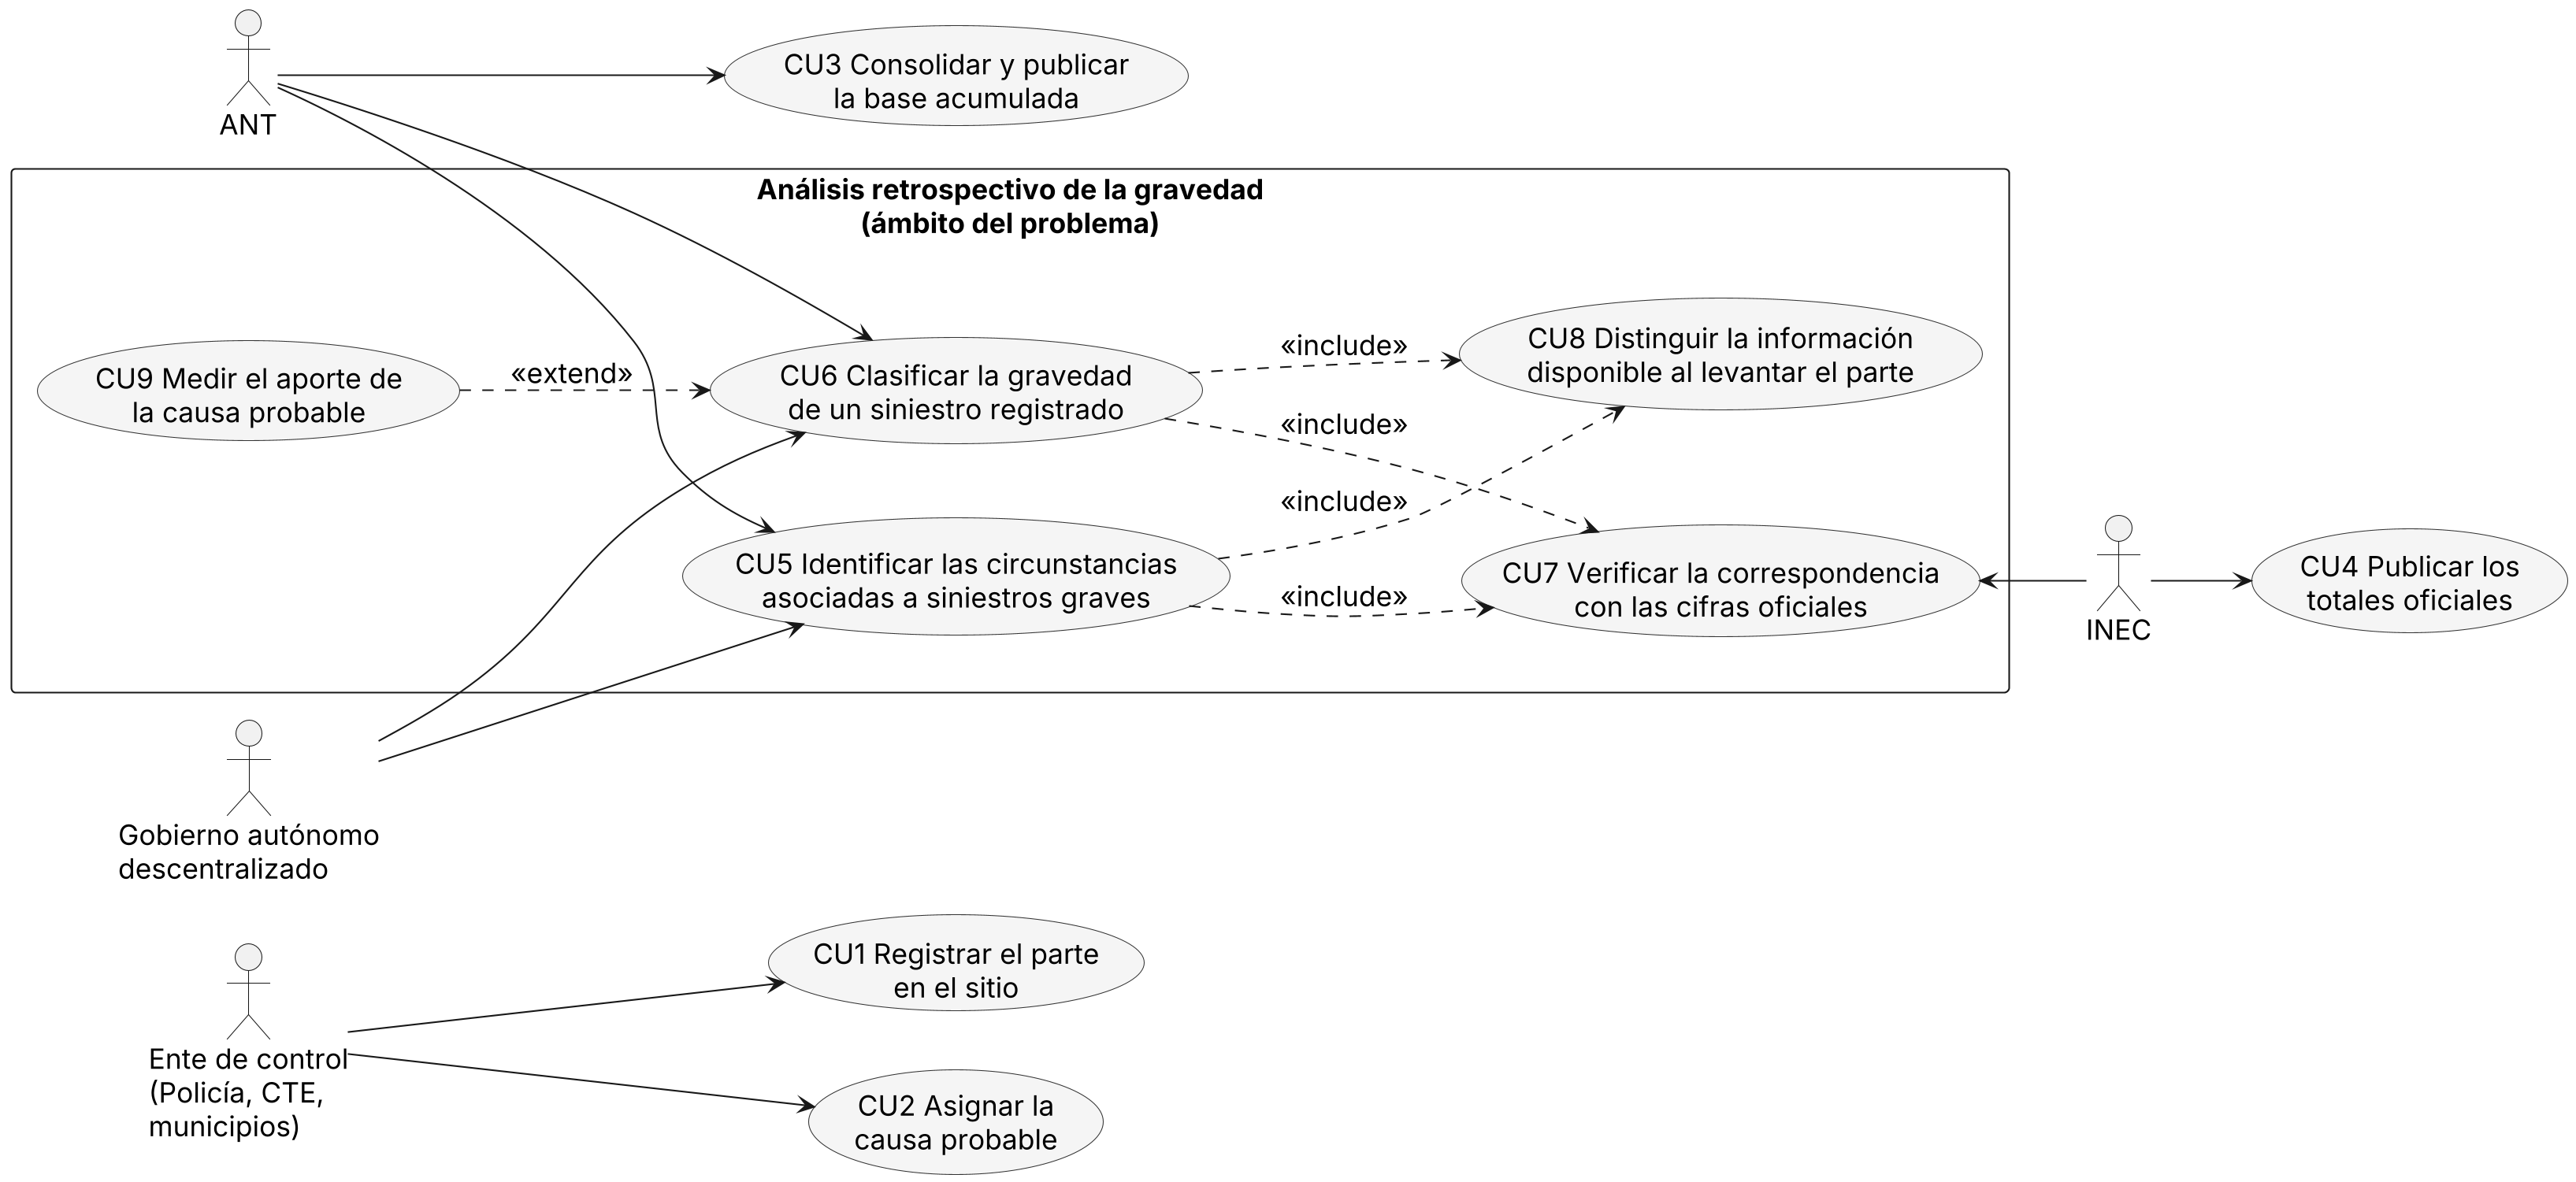
\includegraphics[width=1.10\textwidth]{figuras/M1_casos_de_uso.png}}
\caption{M1. Casos de uso del análisis retrospectivo de la gravedad.}
\label{fig:m1}
\end{figure}

\paragraph{M2. Clases de dominio: qué datos existen y qué papel cumple cada uno.} \texttt{Siniestro} se relaciona uno a uno con \texttt{Ubicación} y con \texttt{CircunstanciaDelEvento}, y uno a muchos con \texttt{VehiculoInvolucrado}; cada siniestro pertenece a un \texttt{EnteDeControl}. Esas cuatro clases forman el conjunto~A. \texttt{CausaProbable} se asocia con cero o una por siniestro y forma el conjunto~B, porque se asigna al investigar. \texttt{Participante}, de uno a 43 por siniestro, queda excluida: su atributo \texttt{condicion} contiene el valor \texttt{fallecido}. De los participantes se deriva \texttt{Resultado}, y de este la \texttt{Etiqueta}; ambos son el desenlace y nunca son entrada. Las coordenadas, la dirección y el nombre de la vía también se excluyen por privacidad. Los estereotipos de la figura indican el papel de cada clase.

\begin{figure}[htbp]
\centering
\makebox[\textwidth][c]{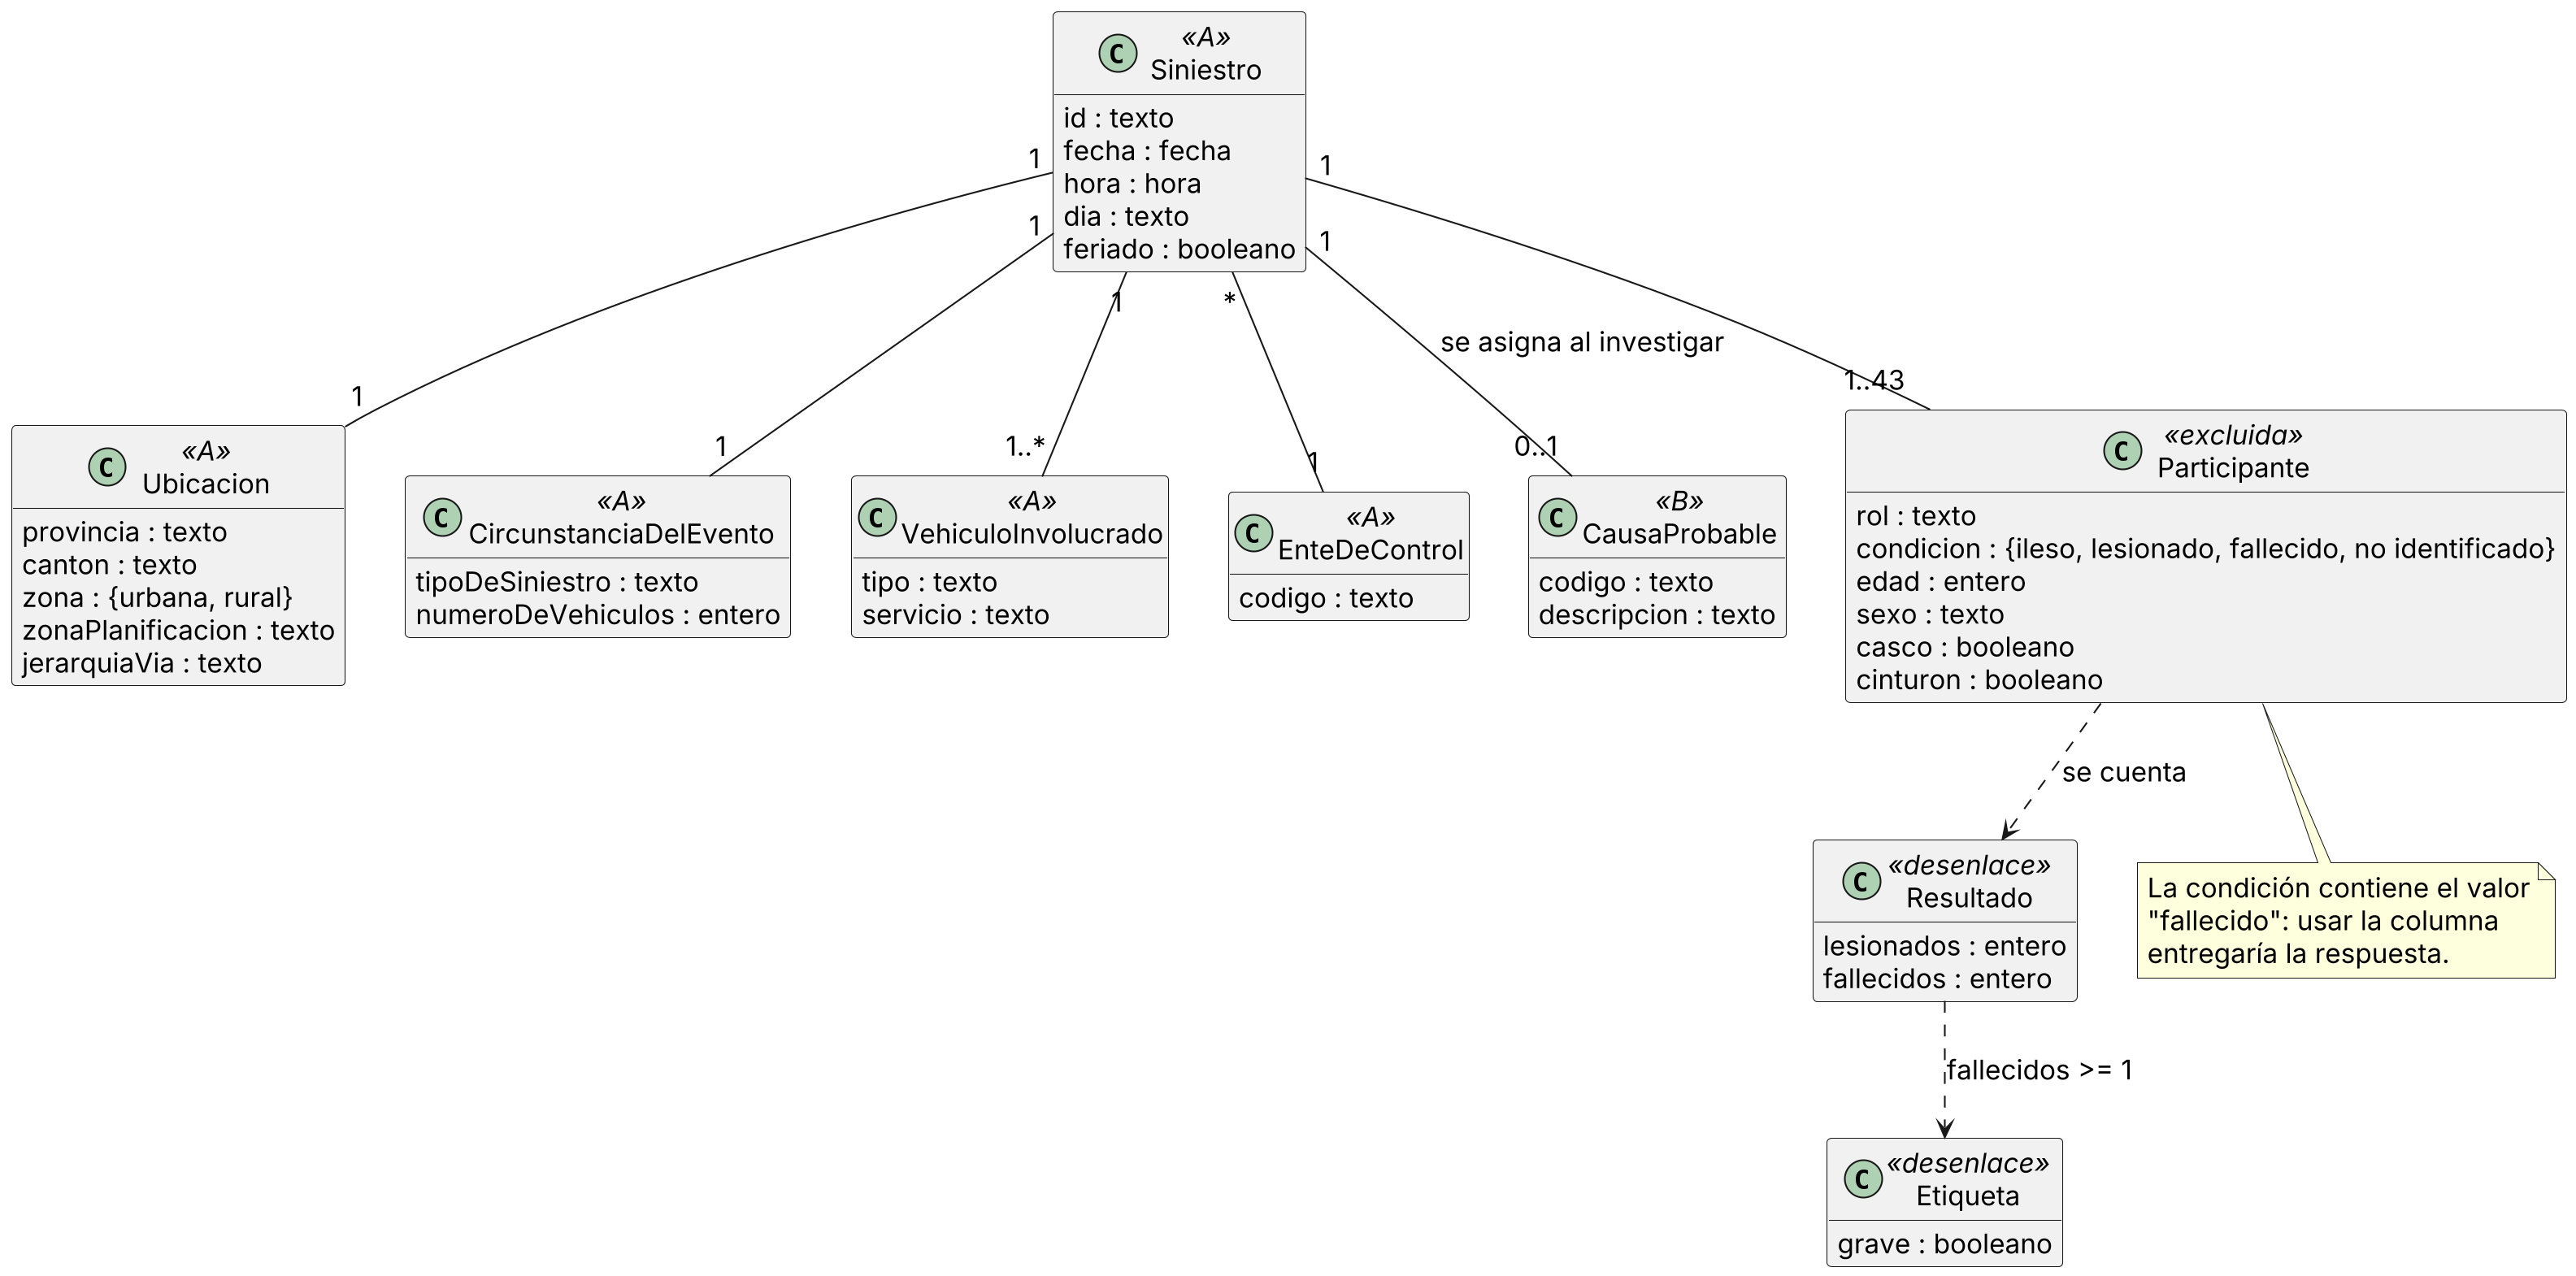
\includegraphics[width=1.08\textwidth]{figuras/M2_clases_de_dominio.png}}
\caption{M2. Clases del dominio del problema y clasificación de sus atributos.}
\label{fig:m2}
\end{figure}

\paragraph{M3. Actividad: cómo se produce y se usa el dato.} El diagrama tiene cuatro carriles. El ente de control atiende el siniestro y levanta el parte con las circunstancias del conjunto~A; si no puede determinar un campo, lo registra como \texttt{ND} o no identificado. Luego registra a los participantes y su condición, que constituye el desenlace; si una persona fallece después del evento, sigue registrada como lesionada según la convención de la sección~2.2. Al terminar la investigación asigna la causa probable, que forma el conjunto~B, y envía el parte a la ANT. Esta consolida los partes de los 16 entes de control y publica el archivo acumulado del año, que conserva los defectos de origen descritos en la Tabla~\ref{tab:a3}. El INEC procesa los mismos registros y publica totales trimestrales. El gobierno autónomo descentralizado consulta ambas fuentes, pero los totales no responden qué circunstancias se asocian con los fallecidos en sitio; esa necesidad no cubierta es el problema que se analiza.

\begin{figure}[htbp]
\centering
\makebox[\textwidth][c]{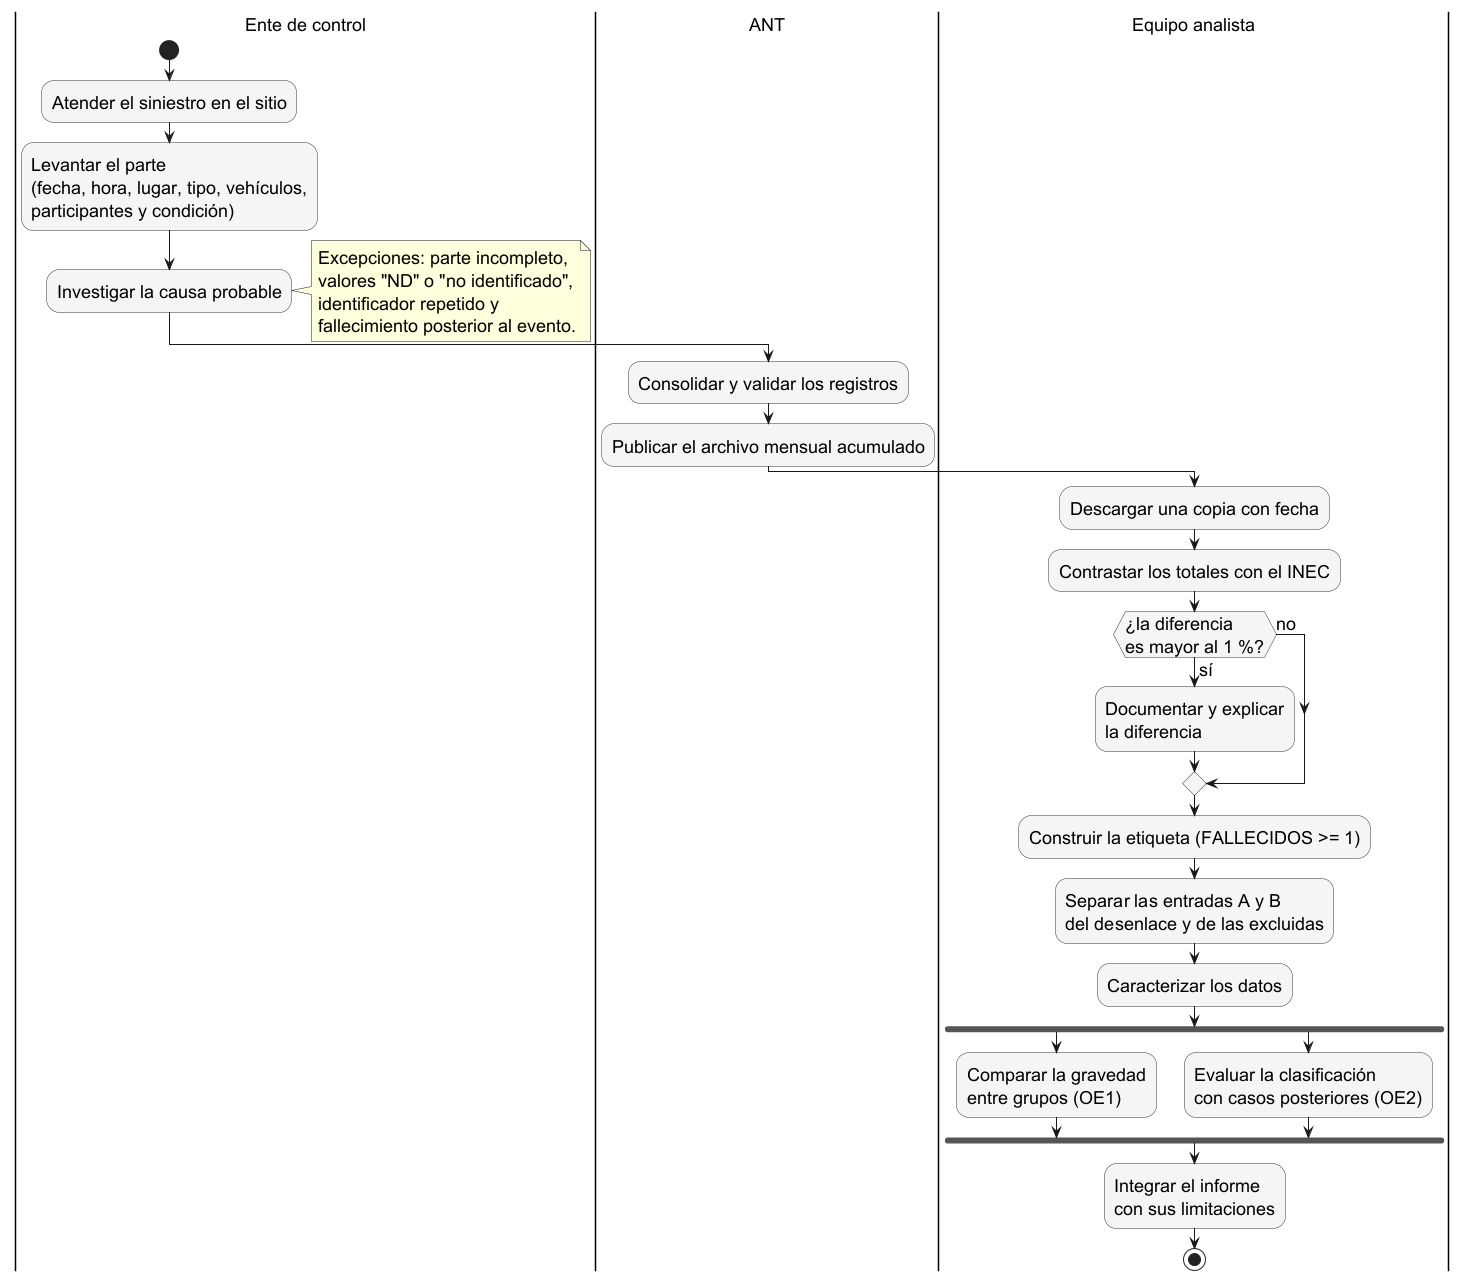
\includegraphics[width=1.10\textwidth,height=0.80\textheight,keepaspectratio]{figuras/M3_actividad.png}}
\caption{M3. Producción, consolidación y uso del dato del siniestro.}
\label{fig:m3}
\end{figure}

\paragraph{M4. Estados: cuándo existe cada información.} Un siniestro ocurre, es atendido en el sitio y llega al estado \emph{parte levantado}, en el que se conocen la fecha, la hora, el lugar, el tipo de siniestro y los vehículos. Después pasa a \emph{causa asignada}, luego a \emph{consolidado por la ANT} y finalmente a \emph{publicado con corte al 30 de septiembre de 2026}. El instante del análisis retrospectivo es \emph{parte levantado}. El recuento de víctimas existe ya en ese estado, pero no puede usarse como entrada porque es lo que se quiere clasificar.

\begin{figure}[htbp]
\centering
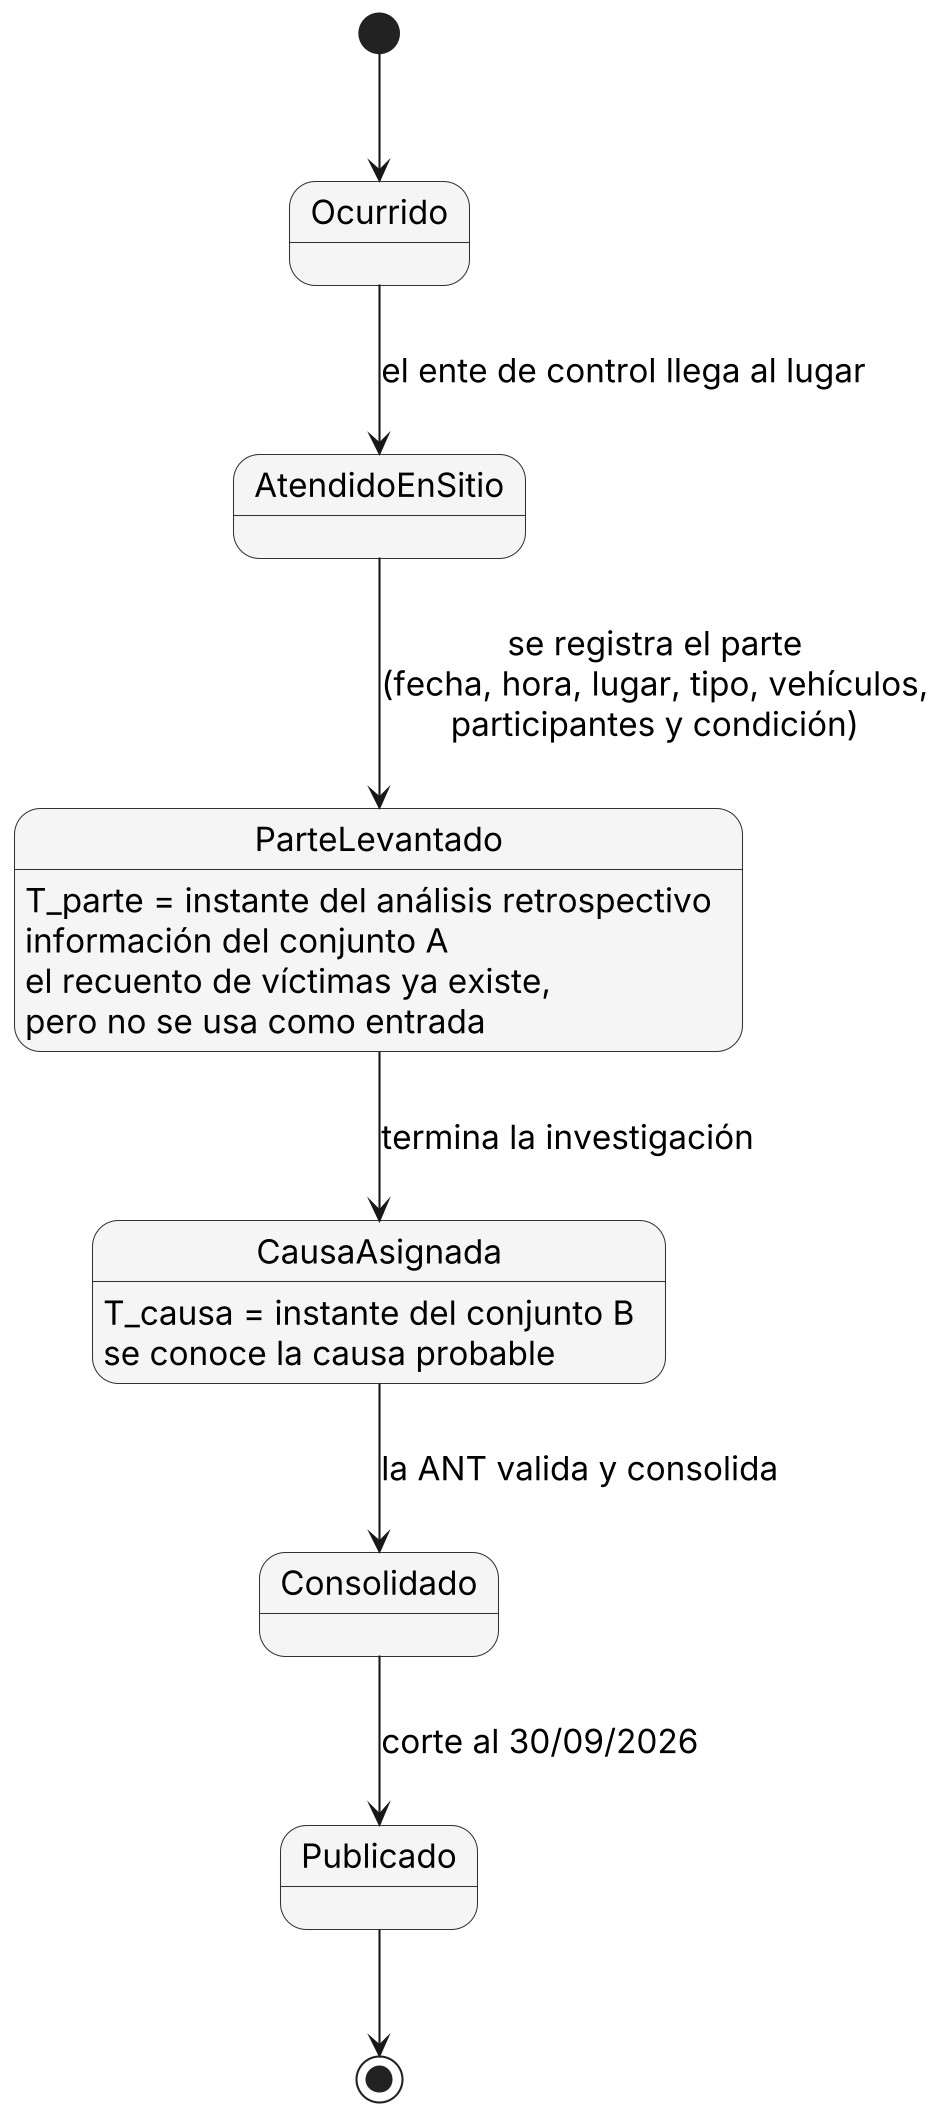
\includegraphics[width=0.92\textwidth,height=0.62\textheight,keepaspectratio]{figuras/M4_estados.png}
\caption{M4. Estados del registro e información disponible en cada uno.}
\label{fig:m4}
\end{figure}


\paragraph{M5. Secuencia: cómo circula la información.} El ente de control envía a la ANT el parte con las circunstancias y la condición de los participantes, y más tarde la causa probable. Si una persona fallece después del evento, el registro no cambia y la persona sigue como lesionada. La ANT consolida los partes, entrega los registros al INEC y publica el archivo acumulado; el INEC publica los totales trimestrales. Con ambas fuentes, el gobierno autónomo descentralizado busca qué circunstancias se asocian con los fallecidos en sitio, y en los territorios con menos de 30 siniestros la proporción local no es confiable. La secuencia termina en la misma necesidad que M3: el archivo contiene el desenlace, pero no la relación entre circunstancias y gravedad.

\begin{figure}[htbp]
\centering
\makebox[\textwidth][c]{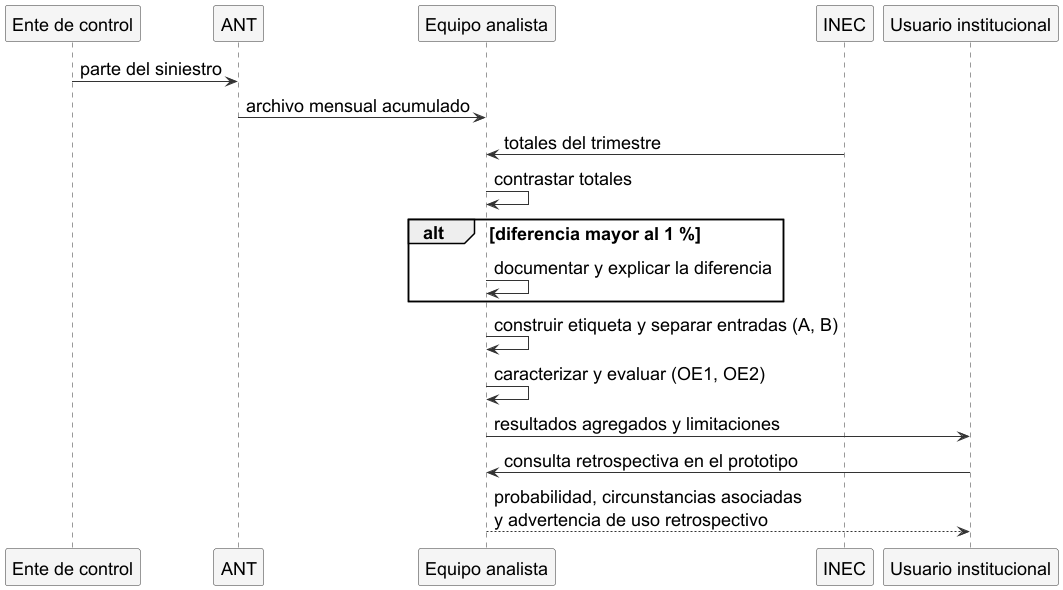
\includegraphics[width=1.05\textwidth]{figuras/M5_secuencia.png}}
\caption{M5. Secuencia de mensajes entre los actores.}
\label{fig:m5}
\end{figure}

\subsection{Escenarios de los casos de uso}
\label{sec:escenarios}

Cada caso de uso de M1 se describe con un escenario principal y uno alterno o de excepción tomado del archivo real, con las mismas excepciones que M3. CU1 a CU4 quedan fuera del límite del análisis, pero se describen porque producen el dato del que dependen los demás; CU7 y CU8 no tienen actor directo porque los incluyen CU5 y CU6, y CU9 se activa desde CU6.

\newcommand{\escenario}[7]{%
\begin{table}[H]
\centering
\small
\caption{#1}
\begin{tabularx}{\textwidth}{>{\raggedright\arraybackslash\bfseries}p{2.9cm}X}
\toprule
Actor & #2 \\
Objetivo & #3 \\
Precondición & #4 \\
\midrule
Escenario 1 (principal) & #5 \\
Escenario 2 (alterno) & #6 \\
\midrule
Postcondición & #7 \\
\bottomrule
\end{tabularx}
\end{table}}

\escenario{CU1. Registrar el parte en el sitio}
{Ente de control (Policía Nacional, CTE, entidades municipales).}
{Dejar constancia del siniestro con sus circunstancias, vehículos, participantes y condición.}
{Ocurrió un siniestro y el ente de control lo atiende en el sitio.}
{(1) El ente atiende el siniestro. (2) Registra fecha, hora, lugar, tipo de siniestro y vehículos. (3) Registra a los participantes y su condición. (4) Envía el parte a la ANT.}
{\emph{Campo sin dato o fallecimiento posterior.} Si no puede determinar un campo, como la jerarquía de la vía o el tipo de vehículo, lo registra como \texttt{ND} o no identificado. Si una persona fallece después del evento, en la CTE sigue registrada como \texttt{LESIONADO}.}
{El siniestro queda registrado y el recuento de víctimas ya está definido.}

\escenario{CU2. Asignar la causa probable}
{Ente de control.}
{Determinar la causa más probable del siniestro una vez investigado el hecho.}
{El parte fue levantado (CU1).}
{(1) El ente investiga el hecho. (2) Asigna una de las 26 causas probables del catálogo de la ANT. (3) Completa el parte con el código y la descripción de la causa.}
{\emph{Causa que refleja el desenlace.} La causa se asigna cuando ya se conoce lo ocurrido, por ejemplo un peatón que cruza sin respetar la señalización. Por eso la causa no forma parte del conjunto~A y se trata por separado en el conjunto~B.}
{El siniestro tiene una causa asignada, posterior al levantamiento del parte.}

\escenario{CU3. Consolidar y publicar la base acumulada}
{ANT.}
{Unir los partes de los entes de control y publicar el archivo acumulado del año.}
{La ANT recibió los partes del periodo.}
{(1) La ANT recibe los partes de los 16 entes de control. (2) Los consolida. (3) Publica el archivo acumulado con corte al 30 de septiembre de 2026.}
{\emph{Republicación del acumulado.} Cada mes el archivo se publica de nuevo con todos los meses anteriores y puede incluir registros añadidos o corregidos. Por eso cada copia se identifica por su fecha de descarga (H-06).}
{El archivo está disponible con sus defectos de origen (Tabla~\ref{tab:a3}).}

\escenario{CU4. Publicar los totales oficiales}
{INEC.}
{Publicar las cifras oficiales de siniestros, lesionados y fallecidos por trimestre.}
{El INEC recibió los registros consolidados de la ANT.}
{(1) El INEC procesa los registros. (2) Publica los totales del primer trimestre de 2026: 4.789 siniestros, 4.032 lesionados y 603 fallecidos \cite{ref1}.}
{\emph{Periodo sin boletín.} Si el periodo que se quiere verificar no tiene boletín trimestral, se usa otra cifra oficial del mismo periodo, como la de la ANT para enero a mayo: 8.718 siniestros \cite{ref7}.}
{Existen totales oficiales con los que puede verificarse el archivo.}

\escenario{CU5. Identificar las circunstancias asociadas a siniestros graves}
{ANT y gobiernos autónomos descentralizados; entes de control como lectores.}
{Conocer cómo varía la proporción de siniestros graves entre grupos definidos con el conjunto~A (OE1).}
{El archivo fue verificado (CU7) y la información disponible está delimitada (CU8).}
{(1) Se agrupan los siniestros por una circunstancia del conjunto~A, por ejemplo el tipo de siniestro. (2) Para cada grupo se obtienen el número de casos, la proporción de graves y una medida de incertidumbre. (3) Los grupos se ordenan: van del 3,0\,\% en colisiones al 45,8\,\% en arrollamientos.}
{\emph{Grupo o territorio con pocos casos.} Si un grupo, como un cantón o una causa poco frecuente, tiene menos de 30 casos, su proporción es inestable y no se reporta como de mayor gravedad.}
{Las diferencias entre grupos quedan descritas como asociaciones, con su número de casos e incertidumbre.}

\escenario{CU6. Clasificar la gravedad de un siniestro registrado}
{ANT y gobiernos autónomos descentralizados.}
{Determinar si un siniestro ya registrado tuvo al menos un fallecido en sitio, usando solo las circunstancias del parte (OE2).}
{El archivo fue verificado (CU7) y la información disponible está delimitada (CU8).}
{(1) Se toma un siniestro ya registrado. (2) Se usan solo sus variables del conjunto~A. (3) Se obtiene la probabilidad de que registre al menos un fallecido en sitio. (4) La clasificación se compara con las dos referencias sencillas en casos posteriores en el tiempo.}
{\emph{Siniestro con información incompleta.} Si el parte tiene campos en \texttt{ND}, como ocurre con la jerarquía de la vía en el 66,4\,\% de los registros, ese valor se trata como una categoría propia y la clasificación se apoya en el resto de las circunstancias.}
{El siniestro queda clasificado de forma retrospectiva, sin anticipar siniestros futuros.}

\escenario{CU7. Verificar la correspondencia con las cifras oficiales}
{Sin actor directo; lo incluyen CU5 y CU6. El INEC aporta los totales.}
{Comprobar que el archivo corresponde a la fuente oficial (CA-01).}
{Existen una copia del archivo con fecha de descarga y totales oficiales de un periodo común (CU4).}
{(1) Se cuentan siniestros, lesionados y fallecidos del primer trimestre en el archivo: 4.789, 4.032 y 603. (2) Se comparan con los del INEC. (3) La diferencia es del 0\,\% y el archivo se considera válido.}
{\emph{Diferencia mayor al 1\,\%.} Si algún total difiere en más del 1\,\%, la diferencia y su posible explicación, como una republicación del acumulado, se documentan antes de interpretar cualquier resultado.}
{La correspondencia del archivo con las cifras oficiales queda documentada.}

\escenario{CU8. Distinguir la información disponible al levantar el parte}
{Sin actor directo; lo incluyen CU5 y CU6.}
{Separar lo que existe al levantar el parte de lo que aparece después o contiene el desenlace (CA-02).}
{Se conoce el catálogo de las 374 columnas del archivo.}
{(1) Las circunstancias del evento forman el conjunto~A. (2) La causa probable se separa en el conjunto~B. (3) \texttt{FALLECIDOS} y \texttt{LESIONADOS} se tratan como desenlace. (4) \texttt{CONDICION\_1} a \texttt{CONDICION\_43} se excluyen porque coinciden con el recuento de víctimas en el 100\,\% de los registros. (5) Los campos personales y de ubicación exacta se excluyen.}
{\emph{Valores inconsistentes o identificador repetido.} Diez registros escriben \texttt{colisión} en minúscula, 14 tienen valor~0 en la jerarquía de la vía y un identificador aparece en dos siniestros de fechas distintas. Las escrituras se unifican, el 0 se agrupa con \texttt{ND} y ambas filas del identificador repetido se conservan sin usarlo como llave.}
{Cada variable tiene un papel definido: entrada de A, entrada de B, desenlace o excluida.}

\escenario{CU9. Medir el aporte de la causa probable}
{Sin actor directo; extiende a CU6.}
{Cuantificar cuánto añade la causa probable a la clasificación y con qué riesgo.}
{Existe la clasificación con el conjunto~A (CU6).}
{(1) A las circunstancias del conjunto~A se agrega la causa probable. (2) Con los mismos siniestros y el mismo orden temporal, se compara cuánto permite distinguir cada conjunto los siniestros graves. (3) La diferencia se reporta como aporte de la causa.}
{\emph{Mejora muy grande con el conjunto~B.} Si B supera ampliamente a A, la mejora se interpreta con cautela, porque la causa puede reflejar el desenlace, y el conjunto~A se mantiene como escenario principal.}
{El aporte de la causa probable queda medido y separado del escenario principal.}

\subsection{Matrices de trazabilidad}
\label{sec:trazabilidad}

La primera matriz relaciona cada objetivo con los requerimientos de la sección~7, los datos de la sección~6, los actores de la sección~4, las restricciones de la sección~8, los criterios de la sección~9 y los modelos de esta sección. Las celdas con varios identificadores indican que un mismo elemento interviene en más de un objetivo.

\begin{longtable}{p{1.3cm}p{2.7cm}p{2.0cm}p{2.0cm}p{1.6cm}p{1.8cm}p{1.8cm}}
\caption{Trazabilidad entre objetivos, requerimientos, datos, actores, restricciones, criterios y modelos}
\label{tab:trazabilidad}\\
\toprule
Obj. & Requerimientos & Datos & Actores & Restr. & Criterios & Modelos \\
\midrule
\endfirsthead
\multicolumn{7}{l}{\footnotesize\itshape (continuación)}\\
\toprule
Obj. & Requerimientos & Datos & Actores & Restr. & Criterios & Modelos \\
\midrule
\endhead
\bottomrule
\endfoot
General & RF-01, RF-02, RF-03, RNF-01 & Archivo de la ANT completo & ANT, INEC & R-04, R-05, R-10 & CA-01, CA-08 & M1 (CU7), M3, M5 \\
OE1 & RF-04, RF-05, RF-10, RNF-03, RNF-05 & Conjunto A y etiqueta & ANT, entes y gobiernos locales & R-04, R-07, R-08 & CA-03 & M1 (CU5), M2, M3 \\
OE2 & RF-03, RF-06, RF-07, RF-08, RF-09, RNF-01, RNF-02, RNF-04 & Conjuntos A y B y etiqueta & ANT, gobiernos locales & R-01, R-02, R-03, R-06 & CA-02, CA-04 a CA-07 & M1 (CU6, CU8, CU9), M2, M4 \\
OE3 & RF-11, RNF-04 & Resultados del modelo seleccionado & ANT, gobiernos locales & R-01, R-08, R-09 & CA-09 & M1 (CU6) \\
\end{longtable}

La segunda matriz desagrega la anterior por requerimiento: cada fila indica el caso de uso que lo origina, el dato que lo alimenta, el actor del que depende, el criterio que lo comprueba y el modelo donde aparece.

\begin{longtable}{p{1.3cm}p{1.7cm}p{3.6cm}p{2.3cm}p{2.1cm}p{1.8cm}}
\caption{Trazabilidad por requerimiento}
\label{tab:trazabilidad-rf}\\
\toprule
Req. & CU & Dato & Actor & Criterio & Modelo \\
\midrule
\endfirsthead
\multicolumn{6}{l}{\footnotesize\itshape (continuación)}\\
\toprule
Req. & CU & Dato & Actor & Criterio & Modelo \\
\midrule
\endhead
\bottomrule
\endfoot
RF-01 & CU7 & Totales del primer trimestre del archivo y del INEC & ANT, INEC & CA-01 & M1, M5 \\
RF-02 & CU6, CU8 & \texttt{FALLECIDOS} & ANT por la convención de registro & CA-01, CA-08 & M2, M4 \\
RF-03 & CU8 & \texttt{CONDICION\_k}, \texttt{FALLECIDOS}, \texttt{LESIONADOS} & Entes de control & CA-02 & M2, M4 \\
RF-04 & CU8 & Jerarquía de la vía, tipo de vehículo, tipo de siniestro (Tabla~\ref{tab:a3}) & Entes de control & CA-02, CA-03 & M3 \\
RF-05 & CU5 & Conjunto A y etiqueta & ANT, gobiernos locales & CA-03 & M1, M5 \\
RF-06 & CU6 & \texttt{FECHA} y etiqueta & ANT, gobiernos locales & CA-05, CA-07 & M4 \\
RF-07 & CU6, CU9 & Conjuntos A y B & ANT, gobiernos locales & CA-04 & M1, M2 \\
RF-08 & CU6 & Etiqueta de la prueba (ago--sep) & ANT, gobiernos locales & CA-04, CA-05 & M1 \\
RF-09 & CU6 & Probabilidades y etiqueta & ANT, gobiernos locales & CA-06 & M1 \\
RF-10 & CU5, CU6 & Resultados de OE1 y OE2 & ANT, gobiernos locales & CA-03, CA-08 & M1, M5 \\
RF-11 & CU6 & Modelo seleccionado & ANT, gobiernos locales & CA-09 & M1 \\
RNF-01 & CU7 & Copia del archivo con fecha de descarga & ANT & CA-01, CA-09 & M3 \\
RNF-02 & CU6 & Tramos temporales (Tabla~\ref{tab:a6}) & ANT, gobiernos locales & CA-04, CA-06 & M4 \\
RNF-03 & CU8 & Defectos de la Tabla~\ref{tab:a3} & Entes de control & CA-02 & M3 \\
RNF-04 & CU5, CU6 & Resultados & Gobiernos locales & CA-08 & M1 \\
RNF-05 & CU5, CU6 & Resultados agregados & Gobiernos locales & CA-03 & M5 \\
\end{longtable}

\section{Caracterización de los datos y de la información requerida}

\subsection{Fuente y estructura}

Los datos provienen del archivo \emph{BDD\_Septiembre\_2026} de la ANT \cite{ref2}, formado por registros administrativos que levantan 16 entes de control en el lugar del siniestro. No son una muestra diseñada para estudiar la gravedad, y esa condición limita desde el inicio lo que puede concluirse. El archivo tiene 17.236 filas y 374 columnas, alrededor de 6,4 millones de celdas. De esas columnas, 301 describen a participantes ---siete campos para hasta 43 participantes por siniestro--- y las 73 restantes describen el evento y los vehículos; la columna \texttt{RANGO DE EDAD} aparece suelta dentro del bloque de participantes y no lleva sufijo. Como la mediana es de dos participantes por siniestro, las columnas de participantes están vacías en un 95,0\,\% y el 82,6\,\% de todas las celdas está vacío (Tabla~\ref{tab:a1}; Anexo~B).

El libro incluye además hojas auxiliares con los catálogos de causa probable, tipo de siniestro, tipo de vehículo y víctimas. Esas hojas funcionan como diccionario y fueron necesarias para interpretar la convención de fallecidos descrita en la sección~2.2; todas las cifras de esta sección se obtuvieron con el procedimiento del Anexo~B sobre la hoja \texttt{BDD\_2026}.

\subsection{Etiqueta, desbalance y variación en el tiempo}

Con la definición de la sección~2.2, 1.656 siniestros son graves (9,61\,\%). La mayoría registra un solo fallecido y solo 159 tienen dos o más (Tabla~\ref{tab:a1}). Esa clase minoritaria no está repartida de forma pareja en el tiempo: el número de graves por mes es casi constante, entre 172 y 196, pero el total de siniestros crece de 1.510 a 2.242. Como consecuencia, la proporción baja de 11,6\,\% en enero a 8,8\,\% en septiembre (Tabla~\ref{tab:a2}; Anexo~B).

Al mismo tiempo cambia la composición de los registros. Los partes de la Policía Nacional pasan de representar el 17,4\,\% del total en enero a un rango de 26,4\,\% a 28,9\,\% entre agosto y septiembre. La causa de ese cambio no está verificada y puede deberse a cobertura, a forma de registro o a un cambio real en la siniestralidad. Por eso se trata como un posible sesgo de registro o deriva temporal, no como una tendencia de seguridad vial. Por eso la evaluación respeta el orden temporal (sección~9).

\subsection{Calidad: valores faltantes y categorías desconocidas}

Las variables que describen el evento ---fecha, hora, provincia, cantón, zona, tipo de siniestro, causa y ente de control--- no tienen valores vacíos. Las limitaciones están en otras variables. La jerarquía y la ubicación de la vía valen \texttt{ND} en el 66,4\,\% de los registros; el 22,5\,\% no identifica el tipo del primer vehículo. Ambas aportan poca información y se tratan como categorías propias en lugar de imputarse.

Hay además defectos menores que exigen reglas explícitas (Tabla~\ref{tab:a3}; Anexo~B): diez registros escriben \texttt{colisión} en minúscula, cinco horas están almacenadas como texto, un mismo identificador aparece en dos siniestros de fechas distintas y catorce registros tienen valor~0 en la jerarquía de la vía. No hay filas duplicadas y las coordenadas no presentan vacíos ni valores fuera de un rango plausible, aunque no se usarán por privacidad. Ninguno de estos defectos cambia la etiqueta, pero todos deben quedar documentados para que otra persona obtenga las mismas cifras.

\subsection{Clasificación de las variables según disponibilidad y fuga}

La clasificación siguiente aplica las definiciones de las secciones~2.2 y~2.3 a las columnas del archivo.

\begin{table}[htbp]
\centering
\small
\caption{Variables según disponibilidad, fuga y privacidad}
\label{tab:variables}
\begin{tabularx}{\textwidth}{p{3.1cm}X p{4.6cm}}
\toprule
Grupo & Variables & Tratamiento \\
\midrule
Conjunto A & Fecha, hora y franja horaria, día, feriado, provincia, cantón, zona urbana o rural, zona de planificación, jerarquía de la vía, tipo de siniestro, tipo y servicio de los vehículos, número de vehículos, ente de control & Entrada. El ente de control puede reflejar cobertura (sección~6.6) y la jerarquía de la vía tiene 66,4\,\% de \texttt{ND} \\
Conjunto B & Código y descripción de la causa probable & Entrada solo en el escenario de contraste \\
Desenlace & \texttt{FALLECIDOS}, \texttt{LESIONADOS} & No son entrada: \texttt{FALLECIDOS} construye la etiqueta \\
Excluidas por fuga & \texttt{CONDICION\_1} a \texttt{CONDICION\_43} & Coinciden exactamente con el conteo de víctimas en los 17.236 registros (Tabla~\ref{tab:a4}); usarlas entregaría la respuesta \\
Excluidas por privacidad o ambigüedad & \texttt{EDAD}, \texttt{SEXO}, \texttt{RANGO DE EDAD}, \texttt{CASCO}, \texttt{CINTURON}, \texttt{TIPO\_ID}, \texttt{PARTICIPANTE}, coordenadas, dirección, nombre e identificador de la vía & No se usan, conforme a la restricción R-07 \\
\bottomrule
\end{tabularx}
\end{table}

La exclusión por fuga no es una suposición: el conteo de participantes en condición \texttt{FALLECIDO} coincide con \texttt{FALLECIDOS} en el 100\,\% de los registros, y lo mismo ocurre con \texttt{LESIONADO} y \texttt{LESIONADOS}. Esa evidencia sostiene la decisión D4.

\subsection{Variabilidad de la gravedad entre grupos}

La proporción de siniestros graves difiere lo suficiente entre grupos como para que la caracterización tenga sentido (Tabla~\ref{tab:a5}; Anexo~B). Según el tipo de siniestro va del 3,0\,\% en colisiones y caídas de pasajero al 45,8\,\% en arrollamientos. Es del 14,0\,\% en zona rural frente al 7,1\,\% en zona urbana, y del 13,4\,\% cuando interviene una motocicleta frente al 7,8\,\% cuando no. Entre entes de control, la Policía Nacional registra 16,3\,\% y la ATM de Guayaquil 6,7\,\%; entre causas probables con al menos 100 casos, el rango va del 1,9\,\% al 23,1\,\%. En la Tabla~\ref{tab:a5} se omiten los grupos con menos de 30 casos, de acuerdo con el criterio CA-03.

Estas diferencias son descriptivas y no implican causalidad. Varias de las variables que las producen están relacionadas entre sí ---el tipo de siniestro con el número de vehículos, por ejemplo---, y los grupos pequeños tienen proporciones inestables. Esa es la razón por la cual OE1 exige informar el número de casos y una medida de incertidumbre junto con cada proporción.

\subsection{Sesgos, dependencias y restricciones de uso}

El sesgo principal proviene del registro: el ente de control puede reflejar cobertura y no solo riesgo, de modo que las diferencias entre entes no deben leerse como diferencias entre territorios. Entre las variables hay dependencias que condicionan el análisis. La hora es cíclica, porque las 23:00 y las 00:00 son cercanas; los siniestros próximos en el tiempo y en el espacio comparten condiciones; y el número de vehículos se relaciona con el tipo de siniestro. Todo el análisis se apoya, además, en un solo periodo de nueve meses, sin comparación con otros años.

En cuanto al uso, los datos son públicos pero no se identificó una licencia explícita. Se usarán solo con fines académicos, citando a la ANT, y sin publicar registros individuales, conforme a la restricción R-07.

\subsection{Contraste con cifras oficiales}

Para comprobar que el archivo corresponde a la fuente oficial se contrastan sus totales. Para el primer trimestre de 2026 reúne 4.789 siniestros, 4.032 lesionados y 603 fallecidos, idénticos a los publicados por el INEC \cite{ref1}; para enero a mayo reúne 8.718 siniestros, igual al valor informado por la ANT para ese periodo \cite{ref7} (Tabla~\ref{tab:a4}; Anexo~B). La coincidencia es evidencia preliminar del criterio CA-01 y respalda que la etiqueta equivale a fallecidos en sitio.

\section{Requerimientos del problema}

Los requerimientos funcionales indican lo que debe hacer el sistema que resuelva el problema y los no funcionales, las cualidades que debe tener. Ninguno fija un algoritmo; la columna de origen remite al caso de uso, dato o restricción del que se derivan, y la Tabla~\ref{tab:trazabilidad-rf} completa su relación con actores, datos y criterios. Se marca como alta la prioridad de los que, de incumplirse, invalidarían las conclusiones: la etiqueta, la fuga de información y la evaluación temporal.

\begin{longtable}{p{1.2cm}p{7.0cm}p{2.4cm}p{1.6cm}p{1.2cm}}
\caption{Requerimientos funcionales y no funcionales}
\label{tab:requerimientos}\\
\toprule
Id & Requerimiento & Origen & Obj. & Prior. \\
\midrule
\endfirsthead
\multicolumn{5}{l}{\footnotesize\itshape (continuación)}\\
\toprule
Id & Requerimiento & Origen & Obj. & Prior. \\
\midrule
\endhead
\bottomrule
\endfoot
RF-01 & El sistema debe contrastar los totales de siniestros, lesionados y fallecidos del archivo con los reportes oficiales de un periodo común & CU7; M1, M5 & General & Alta \\
RF-02 & El sistema debe construir la etiqueta con la definición y la fecha de corte de la sección~2.2 & CU6, CU8; \texttt{FALLECIDOS} & General & Alta \\
RF-03 & El sistema debe excluir de las entradas toda variable derivada de las víctimas y registrar la lista final de variables & CU8; M2, M4 & General, OE2 & Alta \\
RF-04 & El sistema debe tratar los valores faltantes, \texttt{ND} y las categorías inconsistentes con reglas explícitas y documentadas & CU8; sección~6.3 & OE1, OE2 & Media \\
RF-05 & El sistema debe reportar por grupo la proporción de graves, el número de casos y una medida de incertidumbre & CU5; conjunto A & OE1 & Alta \\
RF-06 & El sistema debe evaluar la clasificación con casos posteriores en el tiempo a los usados para obtenerla & CU6; M4 & OE2 & Alta \\
RF-07 & El sistema debe comparar al menos cinco tipos de modelos de aprendizaje automático clásico con dos referencias sencillas, con los conjuntos A y B & CU6, CU9; R-03 & OE2 & Alta \\
RF-08 & El sistema debe medir su desempeño sobre la clase grave y no con la exactitud global, que alcanza el 90,4\,\% sin identificar ningún siniestro grave & CU6; R-06 & OE2 & Alta \\
RF-09 & El sistema debe indicar si las probabilidades que estima corresponden a las proporciones observadas & CU6; etiqueta & OE2 & Media \\
RF-10 & El sistema debe presentar las circunstancias más asociadas con la gravedad de forma comprensible para usuarios no especialistas & CU5, CU6 & OE1, OE2 & Media \\
RF-11 & El sistema debe permitir consultar un siniestro registrado y devolver la probabilidad estimada, las circunstancias asociadas y una advertencia de uso retrospectivo & CU6; modelo seleccionado & OE3 & Media \\
RNF-01 & El sistema debe producir las mismas cifras a partir del mismo archivo y la misma versión del procedimiento (reproducibilidad) & CU7; Anexo~B & General, OE2 & Alta \\
RNF-02 & El sistema debe evaluarse con casos no usados para obtener la estimación y con medidas apropiadas al desbalance (confiabilidad) & CU6; etiqueta & OE2 & Alta \\
RNF-03 & El sistema debe registrar toda limpieza o exclusión de datos (trazabilidad) & CU8; sección~6 & OE1 & Media \\
RNF-04 & El sistema debe permitir explicar cada circunstancia que señale como asociada a la gravedad (interpretabilidad) & CU5, CU6 & OE2, OE3 & Media \\
RNF-05 & El sistema debe publicar solo resultados agregados y nunca registros individuales (privacidad) & CU5, CU6; R-07 & OE1 & Alta \\
\end{longtable}

\section{Restricciones y supuestos}

Las restricciones delimitan lo que el proyecto puede hacer. Los supuestos son las condiciones bajo las cuales se formuló el problema y que, de no cumplirse, obligarían a reformularlo.

\paragraph{Restricciones.}

\begin{description}[leftmargin=1.6em,style=nextline,itemsep=0.25em]
\item[R-01. Académica.] No se aceptan funciones, sistemas, interfaces de programación (APIs), \emph{prompts} o servicios ya desarrollados usados como ``cajas negras'' para resolver el problema. El código incluido en el Anexo~B está escrito por el grupo y usa únicamente operaciones de bibliotecas generales.
\item[R-02. Académica.] No se usa aprendizaje profundo con estos datos tabulares.
\item[R-03. Académica.] Un solo algoritmo poco profundo no basta: se comparan al menos cinco tipos de modelos de aprendizaje automático clásico.
\item[R-04. De datos.] Un solo periodo (01/01 al 30/09/2026), registros administrativos y gravedad medida en el lugar de los hechos.
\item[R-05. Temporal.] Los nueve meses disponibles no sostienen conclusiones sobre dos semestres completos ni sobre la variabilidad anual.
\item[R-06. Metodológica.] La evaluación debe ser temporal y usar métricas de la clase grave.
\item[R-07. Legal y de privacidad.] Se usa información pública con fines académicos; se excluyen los campos personales y de ubicación exacta conforme a la Ley Orgánica de Protección de Datos Personales \cite{ref5}, y solo se publican resultados agregados.
\item[R-08. Ética.] Los resultados describen asociaciones, no causas ni responsabilidades. No deben usarse para estigmatizar provincias, cantones o conductores, ni para sancionar.
\item[R-09. Operativa.] El proyecto no produce un sistema operativo para las autoridades. Un uso real exigiría actualizar datos, validar con nuevos periodos y definir responsables.
\item[R-10. De recursos y tiempo.] Equipos personales sin infraestructura especial y un plazo de dos a tres semanas para el desarrollo posterior a esta tarea.
\end{description}

\paragraph{Supuestos.}

\begin{description}[leftmargin=1.6em,style=nextline,itemsep=0.25em]
\item[H-01.] Los entes de control registran de forma sistemática los fallecidos en el sitio; de no ser así, la etiqueta subestima la gravedad en algunas zonas.
\item[H-02.] La fecha, la hora y la ubicación están registradas con corrección razonable.
\item[H-03.] Los criterios de registro son consistentes durante el periodo. La variación descrita en la sección~6.2 pone en duda este supuesto.
\item[H-04.] La definición de fallecido no cambió durante el periodo.
\item[H-05.] La convención de la ANT descrita en la sección~2.2 hace que la etiqueta sea equivalente a ``fallecido en el lugar de los hechos''.
\item[H-06.] El archivo descargado es una copia fiel y estable de la publicación de la ANT.
\end{description}

Entre estas restricciones hay tensiones que conviene explicitar. R-01 puede chocar con RNF-05 si algún modelo resulta costoso de ejecutar; R-05 limita lo que puede concluirse sobre estabilidad; y R-07 excluye información que podría mejorar la clasificación. En los tres casos se prioriza la restricción legal o académica y se declara el costo sobre el desempeño. La tensión entre R-01 y RNF-05, además, debe resolverse en la Tarea~4, cuando se concretice qué bibliotecas de aprendizaje automático se usan y se justifique que su empleo no equivale a delegar la solución en una caja negra.

\section{Criterios de aceptación y evidencia de éxito}

Los criterios permiten decidir si el problema fue abordado sin fijar un algoritmo. Los umbrales se fijan antes de evaluar los resultados de prueba y se mantienen sin cambios; el registro de esa decisión forma parte de la evidencia.

\begin{longtable}{p{1.2cm}p{7.9cm}p{3.4cm}p{1.4cm}}
\caption{Criterios de aceptación y evidencia correspondiente}
\label{tab:criterios}\\
\toprule
Id & Criterio & Evidencia & Obj. \\
\midrule
\endfirsthead
\multicolumn{4}{l}{\footnotesize\itshape (continuación)}\\
\toprule
Id & Criterio & Evidencia & Obj. \\
\midrule
\endhead
\bottomrule
\endfoot
CA-01 & Los totales del primer trimestre de 2026 difieren de los del INEC en menos del 1\,\%, o la diferencia se documenta y explica & Tabla de contraste; resultado preliminar: diferencia del 0\,\% & General \\
CA-02 & Ninguna variable de entrada deriva de la condición, los lesionados o los fallecidos & Revisión de la lista final de variables de la sección~6.4 y de la Tabla~\ref{tab:a4} & OE2 \\
CA-03 & Todo grupo reportado como de mayor gravedad que el conjunto se presenta con su proporción, el número de casos que lo respalda (mínimo 30) y una medida de incertidumbre & Tabla de grupos, con las cifras de la Tabla~\ref{tab:a5} & OE1 \\
CA-04 & Evaluada con casos posteriores en el tiempo, la clasificación supera a las dos referencias sencillas en el área bajo la curva precisión--sensibilidad (PR-AUC), con un intervalo de confianza por remuestreo de la diferencia que no incluya el cero; se reportan sensibilidad y precisión a un umbral declarado & Tabla comparativa de al menos cinco modelos y dos referencias & OE2 \\
CA-05 & El umbral de decisión se fija con la validación de julio y se aplica sin cambios en la prueba de agosto--septiembre & Registro del protocolo de evaluación & OE2 \\
CA-06 & Las probabilidades estimadas se parecen a las proporciones observadas: se reportan la curva de calibración y el puntaje de Brier, con una diferencia absoluta máxima de 0,05 en los rangos con al menos 30 casos & Gráfico y tabla de calibración & OE2 \\
CA-07 & La PR-AUC varía menos de 0,05 entre las ventanas móviles mensuales de la Tabla~\ref{tab:a7}; si no ocurre, se declara la variación en lugar de promediarla & Tabla por ventana & OE2 \\
CA-08 & El informe declara que los resultados son asociaciones, retrospectivos, de nueve meses y con gravedad medida en el sitio & Sección de limitaciones & General \\
CA-09 & El prototipo devuelve probabilidad, circunstancias asociadas y la advertencia de uso retrospectivo; otra persona lo ejecuta con el mismo archivo & Demostración y lista de pasos & OE3 \\
\end{longtable}

La forma de medir cada objetivo queda así completa: OE1 se comprueba con CA-03, OE2 con CA-02 y CA-04 a CA-07, y OE3 con CA-09. CA-01 y CA-08 son transversales porque afectan a los tres. El hecho de que CA-04 exija un intervalo que no incluya el cero no supone dar por ganada la comparación: con 373 siniestros graves en la prueba (Tabla~\ref{tab:a6}), los intervalos serán amplios, y eso debe leerse como un límite de los datos y no como un fallo del método.

\section{Alcance final del problema}

El proyecto resolverá tres cosas para los siniestros de enero a septiembre de 2026: la caracterización de la gravedad entre grupos definidos con las circunstancias del parte (OE1); la evaluación de la clasificación retrospectiva con al menos cinco tipos de modelos de aprendizaje automático clásico frente a dos referencias sencillas, con los conjuntos~A y~B (OE2); y la exposición del modelo seleccionado en una interfaz de consulta de carácter académico (OE3).

Quedan fuera, por estar relacionados pero exceder lo que los datos y el plazo permiten: anticipar siniestros o emitir alertas previas; establecer causas o responsabilidades; estudiar la gravedad de las lesiones y los fallecimientos posteriores al evento; incorporar factores externos como el clima o el fenómeno de El Niño; usar datos personales; comparar con otros años; emplear aprendizaje profundo; y construir un sistema operativo para las autoridades. La exclusión del clima se decidió en la Tarea~2 porque, con un solo periodo y sin información territorial suficientemente detallada, no habría una comparación confiable; queda como trabajo futuro.

El límite temporal merece una precisión adicional. Con enero--septiembre de 2026 es posible revisar la estabilidad entre ventanas del mismo año, pero no sostener afirmaciones sobre dos semestres completos ni sobre variabilidad anual. Cualquier conclusión que se presente con esos alcances sería incompatible con R-05 y con el criterio CA-08.

\begin{thebibliography}{9}

\bibitem{ref1} Instituto Nacional de Estadística y Censos (INEC), ``Siniestros de tránsito trimestral, estadísticas de transporte (ESTRA),'' 2026. [En línea]. Disponible: \url{https://www.ecuadorencifras.gob.ec/siniestros-transito-trimestral/}

\bibitem{ref2} Agencia Nacional de Tránsito (ANT), ``Base de datos de siniestros de tránsito, septiembre 2026,'' Portal de estadísticas de la ANT, 2026. [En línea]. Disponible: \url{https://www.ant.gob.ec/estadisticas/}

\bibitem{ref3} J. K. Morillo Hernández, ``Predicción de la severidad de accidentes de tránsito en Quito mediante inteligencia artificial: un enfoque de clasificación binaria,'' Tesis de maestría, Univ. Tecnológica Indoamérica, Ambato, Ecuador, 2025. [En línea]. Disponible: \url{https://hdl.handle.net/20.500.14809/8191}

\bibitem{ref4} D. Argüello y E. Alcívar, ``Análisis de accidentes de tránsito en el cantón Guayaquil usando Machine Learning,'' Proyecto Integrador, ESPOL, Guayaquil, Ecuador, 2023. [En línea]. Disponible: \url{http://www.dspace.espol.edu.ec/handle/123456789/57462}

\bibitem{ref5} Asamblea Nacional del Ecuador, ``Ley Orgánica de Protección de Datos Personales,'' Registro Oficial, Quinto Suplemento No. 459, Quito, Ecuador, 26 may. 2021.

\bibitem{ref6} Y. Ali, F. Hussain y M. M. Haque, ``Advances, challenges, and future research needs in machine learning-based crash prediction models: A systematic review,'' \emph{Accid. Anal. Prev.}, vol. 194, p. 107378, 2024.

\bibitem{ref7} El Mercurio, ``Siniestros viales, un mal a paso rápido y sin freno en Ecuador,'' Cuenca, Ecuador, 22 jun. 2026. [En línea]. Disponible: \url{https://elmercurio.com.ec/actualidad/2026/06/22/siniestros-viales-paso-rapido-sin-freno-ecuador/}

\bibitem{ref8} Y. Kotsyubynska \emph{et al.}, ``Machine learning and deep learning for predicting traffic crash injury severity: A systematic review and meta-analysis (2014--2025),'' \emph{J. Road Saf.}, vol. 37, no. 1, pp. 46--60, 2026.

\bibitem{ref9} S. Russell y P. Norvig, \emph{Artificial Intelligence: A Modern Approach}, 4.$^a$ ed. Hoboken, NJ, EE. UU.: Pearson, 2021.

\end{thebibliography}


% ------------------------------------------------------------------- anexos
\appendix
\section{Tablas de verificación}

Las tablas de este anexo no se transcribieron a mano: las genera el script del Anexo~B a partir del archivo original de la ANT. Por eso cada cifra citada en la sección~6 remite a una de ellas y, a su vez, a la función que la calcula. En la Tabla~\ref{tab:a5} se omiten los grupos con menos de 30 casos, de acuerdo con el criterio CA-03, y en la Tabla~\ref{tab:a5} las causas se limitan a las que tienen al menos 100 registros. Los códigos de ente de control son los del catálogo de la ANT: PNE (Policía Nacional), CTE (Comisión de Tránsito del Ecuador), ATM (Agencia de Tránsito y Movilidad de Guayaquil) y DMQ (Agencia Metropolitana de Tránsito de Quito); el resto corresponde a entes municipales.

\begin{table}[htbp]
\centering
\small
\caption{Estructura del archivo y construcción de la etiqueta}
\label{tab:a1}
\begin{tabular}{p{8.2cm}p{6.8cm}}
\toprule
Indicador & Valor \\
\midrule
Siniestros (filas) & 17.236 \\
Columnas & 374 \\
Celdas en total & 6.446.264 \\
Columnas que describen el evento & 73 \\
Columnas que describen participantes & 301 \\
Participantes por siniestro (mediana; máximo) & 2; 43 \\
Celdas vacías sobre el total & 82,6\,\% \\
Celdas vacías en las columnas de participantes & 95,0\,\% \\
\addlinespace
Siniestros con al menos un fallecido (graves) & 1.656 (9,61\,\%) \\
Fallecidos por siniestro & 1 $\rightarrow$ 1.497; 2 $\rightarrow$ 126; 3 $\rightarrow$ 23; 4 $\rightarrow$ 6; 5 $\rightarrow$ 3; 6 $\rightarrow$ 1 \\
Siniestros con dos o más fallecidos & 159 \\
Fallecidos registrados en total & 1.863 \\
Lesionados registrados en total & 14.547 \\
Periodo cubierto & 01/01/2026 a 30/09/2026 \\
\bottomrule
\end{tabular}
\par\vspace{2pt}{\footnotesize Fuente: archivo de la ANT [2], hoja BDD\_2026. Cálculo propio (Anexo B).}
\end{table}


\begin{table}[htbp]
\centering
\small
\caption{Siniestros registrados por mes}
\label{tab:a2}
\begin{tabular}{lrrrr}
\toprule
Mes & Siniestros & Graves & \% graves & \% PNE \\
\midrule
Ene & 1.595 & 185 & 11,6\,\% & 17,4\,\% \\
Feb & 1.510 & 172 & 11,4\,\% & 18,4\,\% \\
Mar & 1.684 & 181 & 10,7\,\% & 17,0\,\% \\
Abr & 1.825 & 182 & 10,0\,\% & 18,1\,\% \\
May & 2.104 & 185 & 8,8\,\% & 23,3\,\% \\
Jun & 2.034 & 182 & 8,9\,\% & 24,9\,\% \\
Jul & 2.181 & 196 & 9,0\,\% & 27,0\,\% \\
Ago & 2.242 & 191 & 8,5\,\% & 28,9\,\% \\
Sep & 2.061 & 182 & 8,8\,\% & 26,4\,\% \\
\midrule
Total & 17.236 & 1.656 & 9,6\,\% & 22,9\,\% \\
\bottomrule
\end{tabular}
\par\vspace{2pt}{\footnotesize PNE: Policía Nacional. La última columna muestra qué porcentaje de los registros del mes proviene de ese ente. Cálculo propio (Anexo B).}
\end{table}


\begin{longtable}{p{3.0cm}p{5.4cm}p{4.8cm}}
\caption{Calidad de los registros y tratamiento previsto}\label{tab:a3}\\
\toprule
Aspecto & Evidencia & Tratamiento previsto \\
\midrule
\endfirsthead
\multicolumn{3}{l}{\footnotesize\itshape (continuación)}\\
\toprule
Aspecto & Evidencia & Tratamiento previsto \\
\midrule
\endhead
\bottomrule
\endfoot
Variables del evento sin vacíos & Fecha, hora, provincia, cantón, zona, tipo de siniestro, causa y ente de control & Se usan tal como están \\
Jerarquía y ubicación de la vía & \texttt{ND} en 11.445 registros (66,4\,\%); 14 con valor 0 y 1 vacío & Se trata como categoría propia; el valor 0 se agrupa con \texttt{ND} \\
Tipo del primer vehículo no identificado & 3.870 registros (22,5\,\%) & Se trata como categoría propia y se conserva \\
Tipo de siniestro con dos escrituras & 10 registros con \texttt{colisión} en minúscula & Se unifican con \texttt{COLISIÓN} \\
Hora almacenada como texto & 5 registros & Se convierten a hora y se incorporan a la franja horaria \\
Identificador repetido & 1 identificador (\texttt{MCU00139082026}) en dos siniestros de fechas distintas & Se conservan ambas filas; no se usa el identificador como llave \\
Filas duplicadas & 0 & No se elimina ninguna fila \\
Coordenadas & Sin vacíos y dentro de un rango plausible & No se usan (restricción R-07) \\
\end{longtable}


\begin{table}[!tbp]
\centering
\small
\caption{Contraste con cifras oficiales y verificación de fuga}
\label{tab:a4}
\begin{tabular}{p{4.6cm}p{2.7cm}p{5.0cm}p{1.2cm}}
\toprule
Concepto & Archivo & Referencia & Dif. \\
\midrule
\addlinespace[2pt]\multicolumn{4}{l}{\textit{Contraste con cifras oficiales, enero a marzo de 2026}}\\
Siniestros & 4.789 & INEC: 4.789 & 0\,\% \\
Lesionados & 4.032 & INEC: 4.032 & 0\,\% \\
Fallecidos & 603 & INEC: 603 & 0\,\% \\
\addlinespace
Siniestros, enero a mayo de 2026 & 8.718 & ANT: 8.718 & 0\,\% \\
\addlinespace[2pt]\multicolumn{4}{l}{\textit{Verificación de fuga de información}}\\
Condición \texttt{FALLECIDO} y columna FALLECIDOS & 17.236 de 17.236 & Coincidencia exacta & 100\,\% \\
Condición \texttt{LESIONADO} y columna LESIONADOS & 17.236 de 17.236 & Coincidencia exacta & 100\,\% \\
Categorías de la columna CONDICIÓN & 4 & FALLECIDO, ILESO, LESIONADO, NO IDENTIFICADO & --- \\
\bottomrule
\end{tabular}
\par\vspace{2pt}{\footnotesize Referencias: INEC [1] y ANT [5] para los totales; [2] para el archivo. La segunda parte muestra que la condición de los participantes contiene el desenlace y no puede usarse como entrada. Cálculo propio (Anexo B).}
\end{table}


\begin{longtable}{p{7.5cm}rrr}
\caption{Proporción de siniestros graves por grupo}\label{tab:a5}\\
\toprule
Grupo & n & Graves & \% graves \\
\midrule
\endfirsthead
\multicolumn{4}{l}{\footnotesize\itshape (continuación)}\\
\toprule
Grupo & n & Graves & \% graves \\
\midrule
\endhead
\bottomrule
\endfoot
\addlinespace[2pt]\multicolumn{4}{l}{\textit{Tipo de siniestro}}\\
ARROLLAMIENTOS & 153 & 70 & 45,8\,\% \\
PÉRDIDA DE PISTA & 504 & 113 & 22,4\,\% \\
CHOQUE FRONTAL & 1.142 & 221 & 19,4\,\% \\
VOLCAMIENTOS & 218 & 33 & 15,1\,\% \\
ATROPELLOS & 1.992 & 282 & 14,2\,\% \\
PÉRDIDA DE CARRIL & 2.242 & 289 & 12,9\,\% \\
OTROS & 717 & 61 & 8,5\,\% \\
CHOQUE POSTERIOR & 1.948 & 150 & 7,7\,\% \\
ESTRELLAMIENTOS & 1.977 & 141 & 7,1\,\% \\
ROZAMIENTOS & 564 & 36 & 6,4\,\% \\
CHOQUE LATERAL & 4.858 & 233 & 4,8\,\% \\
COLISIÓN & 472 & 14 & 3,0\,\% \\
CAÍDA DE PASAJERO & 439 & 13 & 3,0\,\% \\
\addlinespace[2pt]\multicolumn{4}{l}{\textit{Zona}}\\
RURAL & 6.297 & 880 & 14,0\,\% \\
URBANA & 10.939 & 776 & 7,1\,\% \\
\addlinespace[2pt]\multicolumn{4}{l}{\textit{Motocicleta}}\\
Con motocicleta & 5.647 & 755 & 13,4\,\% \\
Sin motocicleta & 11.589 & 901 & 7,8\,\% \\
\addlinespace[2pt]\multicolumn{4}{l}{\textit{Ente de control}}\\
MMC & 100 & 23 & 23,0\,\% \\
PNE & 3.951 & 643 & 16,3\,\% \\
MEP & 274 & 38 & 13,9\,\% \\
MQE & 66 & 9 & 13,6\,\% \\
CTE & 3.596 & 334 & 9,3\,\% \\
MLA & 230 & 21 & 9,1\,\% \\
MPO & 157 & 13 & 8,3\,\% \\
MSD & 854 & 67 & 7,8\,\% \\
MAM & 764 & 55 & 7,2\,\% \\
ATM & 3.253 & 219 & 6,7\,\% \\
DMQ & 2.874 & 193 & 6,7\,\% \\
MRI & 196 & 11 & 5,6\,\% \\
MCU & 412 & 15 & 3,6\,\% \\
MMI & 90 & 3 & 3,3\,\% \\
MLO & 392 & 9 & 2,3\,\% \\
\addlinespace[2pt]\multicolumn{4}{l}{\textit{Zona de planificación}}\\
ZONA 1 & 674 & 123 & 18,2\,\% \\
ZONA 2 & 615 & 94 & 15,3\,\% \\
ZONA 5 & 2.939 & 343 & 11,7\,\% \\
ZONA 4 & 2.011 & 211 & 10,5\,\% \\
ZONA 7 & 1.018 & 102 & 10,0\,\% \\
ZONA 3 & 1.749 & 156 & 8,9\,\% \\
ZONA 6 & 1.252 & 98 & 7,8\,\% \\
ZONA 9 & 3.054 & 236 & 7,7\,\% \\
ZONA 8 & 3.924 & 293 & 7,5\,\% \\
\addlinespace[2pt]\multicolumn{4}{l}{\textit{Día de la semana}}\\
DOMINGO & 3.399 & 382 & 11,2\,\% \\
SÁBADO & 3.013 & 322 & 10,7\,\% \\
VIERNES & 2.507 & 232 & 9,3\,\% \\
LUNES & 2.165 & 197 & 9,1\,\% \\
MIÉRCOLES & 1.974 & 173 & 8,8\,\% \\
JUEVES & 2.227 & 191 & 8,6\,\% \\
MARTES & 1.951 & 159 & 8,1\,\% \\
\addlinespace[2pt]\multicolumn{4}{l}{\textit{Feriado}}\\
Feriado & 1.308 & 157 & 12,0\,\% \\
No feriado & 15.928 & 1.499 & 9,4\,\% \\
\addlinespace[2pt]\multicolumn{4}{l}{\textit{Causa probable (solo causas con 100 casos o más)}}\\
No transitar por las aceras o zonas de seguridad destinadas para el efecto & 147 & 34 & 23,1\,\% \\
Malas condiciones de la vía y/o configuración. (iluminación y diseño) & 109 & 21 & 19,3\,\% \\
Conducir en sentido contrario a la vía normal de circulación & 373 & 71 & 19,0\,\% \\
Caso fortuito o fuerza mayor (explosión de neumático nuevo, derrumbe, inundación, caída de puente, árbol, presencia intempestiva e imprevista de semovientes en la vía, etc.) & 215 & 32 & 14,9\,\% \\
Peatón que cruza la calzada sin respetar la señalización existente (semáforos o señales manuales) & 243 & 33 & 13,6\,\% \\
Conducir desatento a las condiciones de tránsito (celular, pantallas de video, comida, maquillaje o cualquier otro elemento distractor) & 4.956 & 605 & 12,2\,\% \\
Conducir vehículo superando los límites máximos de velocidad & 3.331 & 398 & 11,9\,\% \\
No ceder el derecho de vía o preferencia de paso al peatón & 315 & 37 & 11,7\,\% \\
Conducir en estado de somnolencia o malas condiciones físicas (sueño, cansancio y fatiga) & 146 & 16 & 11,0\,\% \\
Presencia de agentes externos en la vía (agua, aceite, piedra, lastre, escombros, maderos, etc.) & 115 & 12 & 10,4\,\% \\
Condiciones ambientales y/o atmosféricas (niebla, neblina, granizo, lluvia) & 305 & 30 & 9,8\,\% \\
No guardar la distancia lateral mínima de seguridad entre vehículos & 363 & 28 & 7,7\,\% \\
Realizar cambio brusco o indebido de carril & 743 & 50 & 6,7\,\% \\
No mantener la distancia prudencial con respecto al vehículo que le antecede & 1.095 & 64 & 5,8\,\% \\
Conduce bajo la influencia de alcohol, sustancias estupefacientes o psicotrópicas y/o medicamentos & 965 & 53 & 5,5\,\% \\
No ceder el derecho de vía o preferencia de paso a vehículos & 730 & 33 & 4,5\,\% \\
No respetar las señales reglamentarias de tránsito. (pare, ceda el paso, luz roja del semaforo, etc) & 2.324 & 92 & 4,0\,\% \\
Bajarse o subirse de vehículos en movimiento sin tomar las precauciones debidas & 369 & 7 & 1,9\,\% \\
\end{longtable}


\begin{table}[htbp]
\centering
\small
\caption{Particiones temporales para la evaluación}
\label{tab:a6}
\begin{tabular}{llrrr}
\toprule
Partición & Meses & Siniestros & Graves & \% graves \\
\midrule
Entrenamiento & Ene a Jun & 10.752 & 1.087 & 10,11\,\% \\
Validación & Jul a Jul & 2.181 & 196 & 8,99\,\% \\
Prueba & Ago a Sep & 4.303 & 373 & 8,67\,\% \\
\bottomrule
\end{tabular}
\par\vspace{2pt}{\footnotesize El umbral de decisión se fija con la validación y se aplica sin cambios en la prueba. Cálculo propio (Anexo B).}
\end{table}


\begin{table}[htbp]
\centering
\small
\caption{Ventanas móviles para revisar la estabilidad}
\label{tab:a7}
\begin{tabular}{lllrrr}
\toprule
Ventana & Meses previos & Mes verificado & Siniestros & Graves & \% graves \\
\midrule
Ventana 1 & Ene--Mar & Abr & 1.825 & 182 & 10,0\,\% \\
Ventana 2 & Ene--Abr & May & 2.104 & 185 & 8,8\,\% \\
Ventana 3 & Ene--May & Jun & 2.034 & 182 & 8,9\,\% \\
Ventana 4 & Ene--Jun & Jul & 2.181 & 196 & 9,0\,\% \\
Ventana 5 & Ene--Jul & Ago & 2.242 & 191 & 8,5\,\% \\
Ventana 6 & Ene--Ago & Sep & 2.061 & 182 & 8,8\,\% \\
\bottomrule
\end{tabular}
\par\vspace{2pt}{\footnotesize Cada ventana contrasta un mes con todos los meses anteriores y conserva el orden temporal. Con estas ventanas se comprueba el criterio CA-07. Cálculo propio (Anexo B).}
\end{table}


\section{Procedimiento de verificación}

Este anexo resume el procedimiento con el que se obtienen las tablas del Anexo~A a partir de la hoja \texttt{BDD\_2026} del archivo de la ANT. Se presenta en pseudocódigo; su implementación usa solo operaciones generales de lectura, agrupación y conteo de datos. Antes de generar las tablas, el procedimiento comprueba las invariantes del paso~9: si el archivo cambiara y las cifras dejaran de coincidir, se detiene en lugar de producir resultados inconsistentes.

\begin{lstlisting}[style=codigo,caption={Procedimiento de verificación y generación de las tablas A1 a A7},label={lst:procedimiento}]
Entrada: hoja BDD_2026 del archivo de la ANT (corte al 30/09/2026)
Salida:  tablas A1 a A7

1. Cargar
   datos <- leer la hoja BDD_2026
   para cada siniestro: grave <- 1 si FALLECIDOS >= 1, si no 0
                        mes   <- mes de FECHA

2. Tabla A1 (estructura y etiqueta)
   contar filas, columnas y celdas vacías
   separar las 301 columnas de participantes (7 campos x 43) de las del evento
   participantes por siniestro: mediana y máximo
   contar graves y siniestros con 2 o más fallecidos

3. Tabla A2 (variación mensual)
   para cada mes: siniestros, graves, % de graves y % de partes de la PNE

4. Tabla A3 (calidad)
   contar ND, valor 0 y vacíos en la jerarquía de la vía
   contar el tipo del primer vehículo no identificado
   contar escrituras distintas del tipo de siniestro y horas en texto
   contar identificadores repetidos y filas duplicadas

5. Tabla A4 (contraste y fuga)
   totales del primer trimestre y de enero a mayo frente a INEC y ANT
   para cada siniestro: comparar el conteo de CONDICION_k = FALLECIDO
                        con FALLECIDOS (y LESIONADO con LESIONADOS)

6. Tabla A5 (gravedad por grupos)
   para cada variable del conjunto A y para la causa probable:
       agrupar y obtener n, graves y % de graves
       omitir grupos con menos de 30 casos (causas: menos de 100)

7. Tabla A6 (tramos temporales)
   referencia = ene-jun; ajuste = jul; verificación = ago-sep
   para cada tramo: siniestros, graves y % de graves

8. Tabla A7 (ventanas móviles)
   para m desde marzo hasta agosto:
       meses previos = ene..m; mes verificado = m+1
       para el mes verificado: siniestros, graves y % de graves

9. Verificar antes de escribir
   exigir 17.236 filas y 1.656 graves
   exigir 4.789 siniestros y 603 fallecidos en el primer trimestre
   exigir coincidencia total entre CONDICION_k y FALLECIDOS
   exigir que ninguna FECHA esté vacía
\end{lstlisting}


% ------------------------------------------------ declaración de uso de IA
% El enunciado la pide al final del reporte: va después de los anexos y
% conserva el número 12.
\renewcommand{\thesection}{\arabic{section}}
\setcounter{section}{11}
\section{Declaración de uso de IA generativa}

\paragraph{Declaración.} Se usó la herramienta Claude (Anthropic) como apoyo en tres tareas: explorar con código la hoja principal del archivo de la ANT (conteos, consistencia y faltantes), comparar alternativas de definición y apoyar la redacción del informe. También se usó para generar los modelos UML y verificar las cifras con el procedimiento del Anexo~B. El grupo revisó cada afirmación y es responsable de la exactitud del contenido; las cifras de la sección~6 pueden reproducirse con ese procedimiento.

\begin{table}[H]
\centering
\small
\caption{Recomendaciones de IA verificadas, corregidas o descartadas}
\label{tab:bitacora}
\begin{tabularx}{\textwidth}{p{0.7cm}X X p{3.0cm}}
\toprule
\# & Recomendación de la IA & Verificación & Resultado \\
\midrule
1 & Excluir las columnas de condición de los participantes porque revelan el desenlace & El conteo de condición \texttt{FALLECIDO} coincide con \texttt{FALLECIDOS} en los 17.236 registros (Tabla~\ref{tab:a4}) & Verificada y adoptada \\
2 & Tratar la causa probable como un conjunto de información separado (B) y no como una variable más & Se contrastó con la retroalimentación recibida y con las proporciones por causa, que van del 1,9\,\% al 23,1\,\% (Tabla~\ref{tab:a5}) & Corregida respecto a la propuesta inicial \\
3 & Describir el conjunto B y las ventanas móviles en términos de entrenar y comparar modelos & En el análisis del problema no se entrena nada; esos elementos son condiciones de evaluación & Corregida; se describen en la sección~9 y en las Tablas~\ref{tab:a6} y~\ref{tab:a7} \\
\bottomrule
\end{tabularx}
\end{table}


\end{document}
